\chapter{Livello Trasporto}
I protocolli del \emph{livello Trasporto} forniscono strumenti per la
comunicazione logica tra processi di \emph{host} differenti e vengono eseguiti dai
sistemi terminali, cioè dal mittente per quello che riguarda l'invio dei dati e
dal destinatario per la ricezione.

\section{Caratteristiche dei servizi offerti}
Tipicamente, al momento dell'invio, i messaggi vengono suddivisi in \emph{segmenti}
e questi sono poi riassemblati al momento della ricezione.

I protocolli che appartengono a questo livello si appoggiano ai servizi
offerti dal \emph{livello Rete} che si occupa di gestire la comunicazione logica
tra \emph{host}. Quindi, il \emph{livello Trasporto} è di fatto un potenziamento del
\emph{livello Rete}.

\bigskip\noindent
I protocolli di \emph{trasporto} principali sono l'\emph{\gls{prot:UDP}} e il
\emph{\gls{prot:TCP}}. Questi due servizi si differenziano per la filosofia
con la quale si approcciano al trasporto dei dati: \emph{best effort} per
l'\emph{UDP} e \emph{affidabile} per il \emph{TCP}. Il \emph{TCP}, infatti, è
un \emph{protocollo connesso}, che garantisce l'arrivo di tutti i \emph{segmenti}
trasmessi permettendo al destinatario di ordinarli e occupandosi anche di gestire
il controllo della congestione e del flusso. D'altra parte, l'\emph{UDP} non
fa nulla di tutto ciò, ma trasmette i \emph{segmenti} cercando di ridurre al
minimo l'overhead; scelta che ovviamente non permette di assicurare l'arrivo
di tutti i dati.

\paragraph{Controllo di congestione e di flusso}
\emph{Controllo della congestione} e \emph{controllo del flusso} sono due
concetti molto diversi che è bene chiarire subito:
\begin{definition}[Controllo della congestione]
    Il controllo della congestione permette di evitare che il mittente
    trasmetta più dati di quelli che la rete può gestire.    
\end{definition}
\begin{definition}[Controllo del flusso]
    Il controllo del flusso permette di evitare che il mittente
    trasmetta più dati di quelli che il destinatario può gestire.
\end{definition}

\subsection{Multiplexing e demultiplexing}
\emph{Multiplexing} e \emph{demultiplexing} sono due operazioni realizzate
rispettivamente dal mittente e dal destinatario.

\noindent
Il \emph{multiplexing} consiste nell'aggiunta ai dati trasmessi dalle
\emph{socket} di un header con le \emph{\gls{glos:PCI}} del \emph{livello
Trasporto}. Le informazioni aggiunte consentono di identificare la \emph{socket
sorgente} e di \emph{destinazione}.
In fase di \emph{demultiplexing} invece, quelle stesse \emph{PCI} vengono usate
per consegnare i \emph{segmenti} ricevuti alla \emph{socket} corretta.

\paragraph{Funzionamento del demultiplexing}
L'\emph{host} riceve i \emph{pacchetti IP} che nel proprio header trasportano
gli \emph{indirizzo IP} sorgente e di destinazione. Ogni \emph{pacchetto IP} ha
come \emph{payload} un \emph{segmento} del \emph{livello Trasporto} nel cui header
sono indicati i \emph{numero di porta} sorgente e di destinazione.
L'\emph{host} utilizza quindi la coppia \emph{indirizzo IP-numero di porta} per
identificare la \emph{socket} alla quale consegnare il \emph{segmento}.
\begin{figure}[h!]
    \centering
    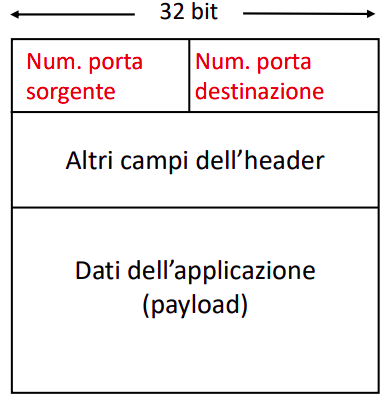
\includegraphics[width=0.4\textwidth]{segmento-livello-trasporto.png}
    \caption{Struttura di un \emph{segmento TCP/UDP}}
\end{figure}

\paragraph{Demultiplexing senza connessione}
Nel caso del protocollo \emph{UDP}, che è un protocollo non connesso, quando
l'\emph{host} riceve un \emph{segmento}, legge i parametri della \emph{socket} di
destinazione (\emph{indirizzo IP-numero di porta} di destinazione) e consegna
il \emph{segmento} a quella \emph{socket}. \emph{Segmenti} proveniente da
processi diversi, ma con gli stessi parametri di destinazione vengono anch'essi
destinati alla medesima.

\paragraph{Demultiplexing con connessione}
Il \emph{TCP}, invece, per identificare una \emph{socket}, usa anche i parametri
di sorgente, quindi l'\emph{host} ricevente utilizza tutti e quattro i parametri per
inviare il \emph{segmento} alla \emph{socket} appropriata. Questo è conseguenza
del fatto che un server può supportare più \emph{socket TPC} contemporaneamente.

\begin{note}
    I server \emph{HTTP} creano \emph{socket} differenti per ogni connessione con
    i client. E, addirittura, con versioni \emph{non-persistenti} dell'\emph{HTTP},
    si ha una \emph{socket} differente per ogni richiesta.
\end{note}

\subsection{Numeri di porta}
Quindi, la destinazione finale di un \emph{segmento} non è un \emph{host}, ma un processo
in esecuzione su un \emph{host}. L'interfaccia tra il \emph{livello Applicativo} e il
\emph{Trasporto} è costituita dal già citato \emph{numero di porta}: un valore
numerico a 16 bit che identifica univocamente un processo all'interno di un
\emph{host}.

I \emph{numeri di porta} per i servizi standardizzati sono noti e sono quindi detti
\emph{well-known}. Si tratta di valori compresi tra $0$ a $1023$ (incluso) che
identificano un processo che fornisce un servizio standardizzato (e.g porta 80
per l'\emph{HTTP}, porta 25 per l'\emph{SMTP}, \dots).

\noindent
I servizi non standard e le connessioni in ingresso a un client utilizzano invece
\emph{numeri di porta} con valori fino a $65535$ ($2^{16}-1$) che sono decisi in
modo automatico dal sistema operativo al momento della creazione di una
\emph{socket} o di instaurazione di una connessione.

\begin{note}
    Le \emph{porte well-known} sono anche dette \emph{statiche}, mentre quelle
    assegnate dal sistema operativo sono dette \emph{effimere}.
\end{note}\noindent
Una cosa importante da tenere a mente è che il \emph{numero di porta} sorgente e
di destinazione non sono quasi mai uguali.
Questo perché i server restano in ascolto su una porta nota ai client, quindi
quando un client contatta, o si connette con il server, lo fa su quella
\emph{porta}. Tuttavia, poiché più processi in esecuzione sullo stesso client
potrebbero contattare lo stesso server, è necessario che ogni processo del
client sia associato ad un \emph{numero di porta} diverso da quello degli altri.
Di conseguenza, non è possibile usare sempre lo stesso \emph{numero di porta}
scelto dal server. In relazione a ciò, è bene chiarire il concetto di
\emph{flusso di dati}:
\begin{definition}[Flusso di dati]
    Un flusso è un gruppo di dati che appartengono alla stessa comunicazione
    logica.
\end{definition}
\begin{note}
    Un'applicazione può aprire molteplici \emph{connessioni} e veicolare
    molti \emph{flussi}.
\end{note}

\section{Protocollo UDP}
Come già accennato, il protocollo \emph{UDP} è orientato alla \quotes{consegna
con minimo sforzo} (\emph{best effort}), col risultato che i \emph{segmenti UDP}
potrebbero non giungere mai a destinazione o arrivare in un ordine diverso da
quello di invio. È anche un protocollo non connesso quindi ogni \emph{segmento}
è gestito in modo indipendente dagli altri.

Se da una parte tutte queste caratteristiche rendono l'\emph{UDP} un protocollo
poco affidabile, lo rendono anche molto meno oneroso in termini di overhead e
ritardi amministrativi: gli header sono più corti, non esiste un ritardo
provocato dall'instaurazione di una connessione, non è necessario mantenere uno
stato della comunicazione e, non facendo controlli di congestione, può inviare
raffiche di dati.

\begin{figure}[h!]
    \centering
    \hspace{-2cm}
    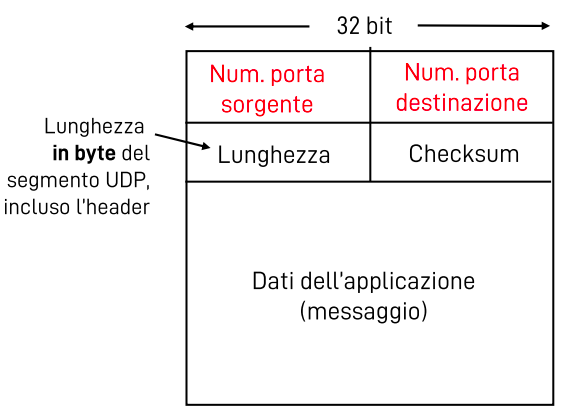
\includegraphics[width=0.4\textwidth]{segmento-UDP.png}
    \caption{Struttura di un \emph{segmento UDP}}
\end{figure}\noindent
Proprio per questa sua \quotes{leggerezza}, l'\emph{UDP} è particolarmente
adatto ad applicazioni multimediali nelle quali piccole perdite sono
tollerabili e che sono sensibili alla frequenza di trasferimento dei dati.
Qualora fosse necessario rendere affidabile una comunicazione basata su
\emph{UDP} è necessario implementare dei controlli al livello di applicazione.

\subsection{Controllo degli errori}
Nell'header di un \emph{segmento UDP} è presente un campo \texttt{Checksum}
che contiene una stringa di bit che il destinatario usa per verificare la
correttezza dei dati ricevuti.

In particolare, il mittente tratta l'intero \emph{segmento} come una sequenza
di parole da 16 bit quindi, somma tutte le parole e calcola il complemento a 1
del risultato. Il valore così ottenuto viene inserito nel campo \texttt{Checksum}
del \emph{segmento}.

Il ricevente, somma di nuovo tutte le parole da 16 bit del \emph{segmento}, incluso
il \texttt{Checksum}. Se il risultato di questa somma è una parola composta da
16 bit uguali a 1, allora è probabile che non ci siano errori\footnote{Vedremo
più avanti perché non se ne può avere la certezza}, altrimenti è certo che i
dati sono danneggiati.

\begin{note}
    Se quando si sommano le parole risulta un bit di riporto sul bit più
    significativo, questo deve essere sommato al risultato. Quindi, il riporto
    va sommato prima di calcolare il complemento a 1.
\end{note}

\begin{note}
    Nessun sistema di rilevamento degli errori è perfetto. Per esempio, nel
    rilevamento di errori con bit di parità (vengono contati i bit pari a 1 e
    impostato a 0 un flag se il numero è pari, altrimenti dispari) si possono
    rilevare soltanto una quantità dispari di bit errati.

    Oppure con il codice a ripetizione (la stessa stringa di bit viene trasmessa
    tre volte) è possibile rilevare e correggere errori se soltanto una stessa
    porzione di una stringa è diversa dalle altre, ma se gli errori sono molti
    non è più possibile essere certi che la correzione sia corretta.
\end{note}

\section{Trasferimento dati affidabile}
Esiste una classe di protocolli detti \emph{\gls{glos:ARQ}} che si propongono
l'obiettivo di recuperare i pacchetti persi. Questo tipo di protocolli usano
pacchetti speciali detti \emph{\gls{glos:ACK}} per notificare al trasmettitore
la corretta ricezione di un pacchetto.
In questa sezione vedremo alcuni esempi di questo tipo di protocolli.

\subsection{Protocollo Stop-and-Wait}
In questo tipo di protocollo, il mittente invia una \emph{\gls{glos:PDU}}
mantenendone però una copia. Quindi, imposta un timeout e attende la ricezione
dell'\emph{ACK} per quella \emph{PDU}. Se entro lo scadere del timeout non riceve
l'\emph{ACK}, ritrasmette la \emph{PDU}, altrimenti controlla, mediante codice
\emph{checksum} che l'\emph{ACK} ricevuto non contenga errori e il numero di
sequenza sia corretto. Se questi controlli sono verificati, allora procede
all'invio della \emph{PDU} successiva.

D'altra parte, quando il destinatario riceve una \emph{PDU}, ne controlla
\emph{checksum} e numero di sequenza. Se sono corretti, invia l'\emph{ACK} e
passa la \emph{\gls{glos:SDU}} ai protocolli del livello superiore, altrimenti
elimina (drop) la \emph{PDU}.
\newpage
\begin{figure}[ht!]
    \centering
    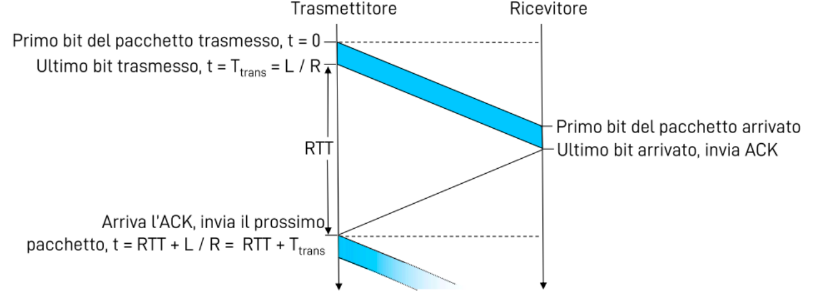
\includegraphics[width=\textwidth]{schema-stop-and-wait.png}
    \caption{Funzionamento protocollo \emph{Stop-and-Wait}}
\end{figure}
\begin{note}
    Nel calcolo del tempo $t$ si è assunta come trascurabile la durata del
    pacchetto \emph{ACK}.
\end{note}

\paragraph{Efficienza}
Se assumiamo $\hyperlink{sym:2}{R}=1Gbit/s$, $\hyperlink{sym:5}{RTT}=30ms$ e
$\hyperlink{sym:1}{L}=8000bit$, il \nameref{ssec:num1} vale $d_{trasferimento}=
\frac{L}{R}=8\mu s$. Quindi, il \emph{throughput} percepito a livello applicazione
è:
\[\emph{Throughput}=\frac{L}{d_{trasferimento}+RTT}=\frac{8000bit}{0.008ms+30ms}=33kByte/s\]
L'efficienza invece, vale:
\[\emph{Efficienza}=\frac{d_{trasferimento}}{d_{trasferimento}+RTT}=0.00027=0.027\%\]
Dai calcoli risulta evidente l'enorme inefficienza di questo protocollo, dovuta
al fatto che per la maggior parte del tempo gli \emph{host} restano in attesa.

\paragraph{Pipelining}
Con la tecnica del \emph{pipelining} il mittente invia più pacchetti alla volta
e tiene traccia del loro numero di sequenza.

\begin{figure}[h!]
    \centering
    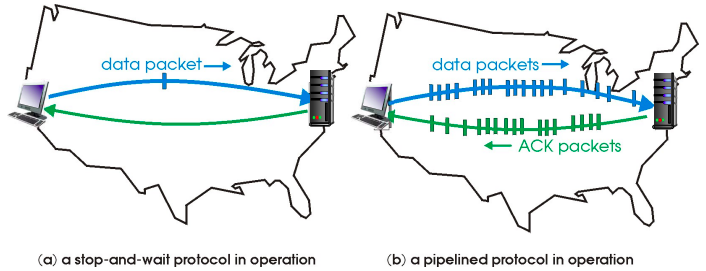
\includegraphics[width=\textwidth]{stop-and-wait-vs-pipelining.png}
    \caption{\emph{Stop-and-Wait} e protocollo con \emph{pipelining}}
\end{figure}\noindent
L'utilizzo del \emph{pipelining} permette di aumentare il \emph{throughput} di un
collegamento. Se, per esempio, si applica il \emph{pipelining} al protocollo
\emph{Stop-and-Wait}, permettendogli quindi di inviare 3 pacchetti prima di
mettersi in attesa, si triplica il \emph{throughput}.

\newpage
\begin{figure}[ht]
    \centering
    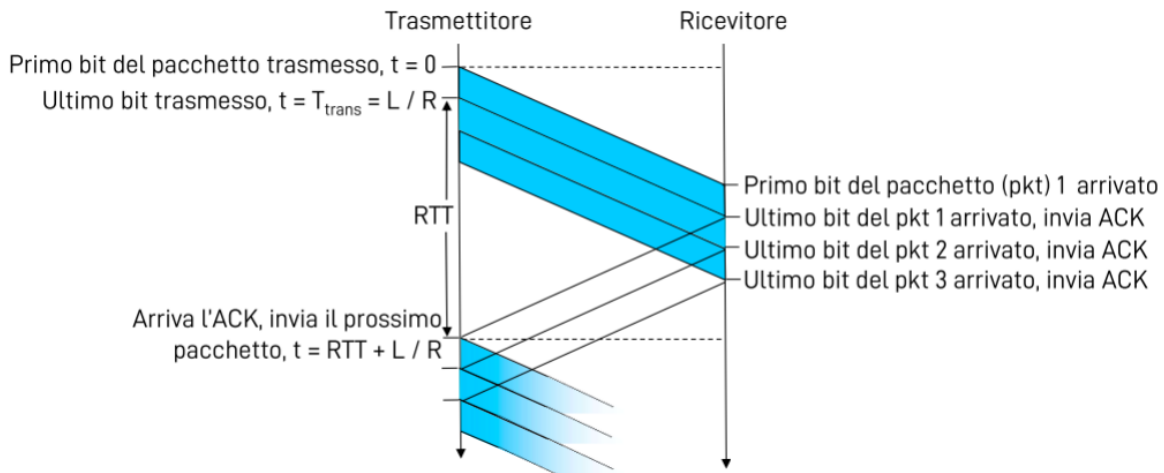
\includegraphics[width=\textwidth]{stop-and-wait-pipelining.png}
    \caption{Funzionamento protocollo \emph{Stop-and-Wait} con \emph{pipelining}}
\end{figure}\noindent
Ricalcolando il \emph{throughput} si può vedere come risulti effettivamente
triplicato:
\[\emph{Throughput}=\frac{3L}{d_{trasferimento}+RTT}=100kByte/s\]
In generale, il \emph{throughput} aumenta di tante volte quanti sono i pacchetti
trasmessi prima della messa in attesa. Tuttavia, ciò vale fino a quando il tempo
necessario a trasmettere quei pacchetti rimane inferiore al \emph{RTT}.

\subsection{Finestre di trasmissione e acknowledgement}
\paragraph{Finestre di trasmissione}
Il numero di pacchetti trasmesso prima della messa in attesa, viene detto
\quotes{\emph{dimensione della finestra}}. Diamo quindi le seguenti definizioni:
\begin{definition}[Finestra di trasmissione - \bm{$W_T$}]
    La finestra di trasmissione, indicata in simboli come $W_T$, è l'insieme di
    PDU che il mittente può trasmettere senza avere ancora ricevuto l'ACK
    corrispondente. La dimensione massima della finestra è limitata dalla
    quantità di memoria allocata dal trasmettitore ed è indicata in simboli come
    $|W_T|$.
\end{definition}
\begin{definition}[Finestra di ricezione - \bm{$W_R$}]
    La finestra di ricezione, indicata in simboli come $W_R$, è l'insieme di
    PDU che il destinatario può ricevere e memorizzare. La dimensione massima
    della finestra è limitata dalla quantità di memoria allocata dal ricevitore.
\end{definition}
\begin{definition}[Puntatore low - \bm{$W_{LOW}$}]
    Il puntatore low, indicato in simboli come $W_{LOW}$, è un puntatore al
    primo pacchetto della finestra di trasmissione $W_T$.
\end{definition}
\newpage
\begin{definition}[Puntatore up - \bm{$W_{UP}$}]
    Il puntatore up, indicato in simboli come $W_{UP}$, è un puntatore
    all'ultimo pacchetto già trasmesso e potrebbe non coincidere con l'ultimo
    pacchetto della finestra di trasmissione.
\end{definition}

\begin{figure}[ht]
    \centering
    \subfloat[\emph{Finestra di trasmissione}]{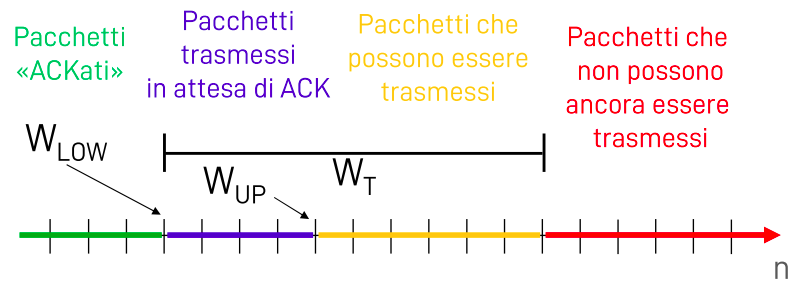
\includegraphics[width=0.8\textwidth]{finestra-trasmissione.png}}
    \hfill
    \subfloat[\emph{Finestra di ricezione}]{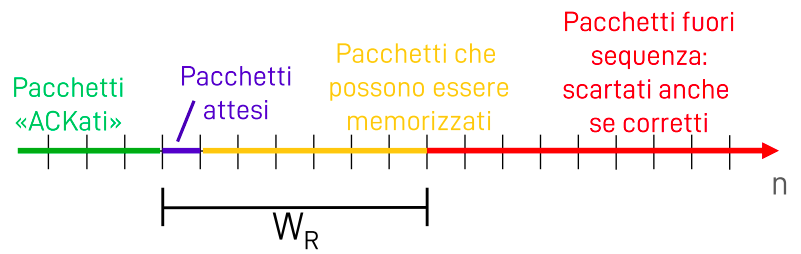
\includegraphics[width=0.8\textwidth]{finestra-ricezione.png}}
    \caption{\emph{Finestre di trasmissione} e \emph{ricezione}}
\end{figure}

\paragraph{Pacchetti di acknowledgement}
Finora abbiamo parlato dei pacchetti \emph{\gls{glos:ACK}} senza specificare
alcun tipo di dettaglio, ma in realtà esistono molteplici tipi di
\emph{acknowledgement}:
\begin{itemize}
    \item \emph{ACK individuale}: indica la corretta ricezione di un pacchetto
    specifico. $ACK(n)$ significa che è stato ricevuto il pacchetto $n$;
    \item \emph{ACK cumulativo}: indica la corretta ricezione di tutti i
    pacchetti fino ad un certo indice. $ACK(n)$ significa che sono stati
    ricevuti correttamente tutti i pacchetti fino al pacchetto $n$ (escluso);
    \item \emph{ACK negativo} (\emph{NACK}): richieda la ritrasmissione di un
    singolo pacchetto. $\emph{NACK}(n)$ significa che il pacchetto $n$ deve
    essere ritrasmesso.
\end{itemize}
Con la tecnica del \quotes{\emph{Piggybacking}} è possibile inserire un
\emph{ACK} in un pacchetto dati.

\subsection{Protocollo Go-back-N}
Nel protocollo \emph{Go-back-N} il mittente può avere fino a $N$ pacchetti
senza \emph{ACK} in pipeline. Il destinatario comunica la corretta ricezione dei
pacchetti mediante \emph{ACK cumulativi} e nel caso di pacchetti non ricevuti non
trasmette alcun \emph{ACK}. Fino a quando non verrà ricevuto il pacchetto mancante,
il protocollo continuerà a scartare tutti i successivi pacchetti ricevuti e, per
ognuno, ritrasmetterà l'ultimo \emph{ACK} inviato.

Il mittente ha un timer per il più vecchio pacchetto non confermato e quando
scade ritrasmette tutti i pacchetti per i quali non ha ricevuto \emph{ACK}.

Per la natura degli \emph{ACK cumulativi}, alcuni dei pacchetti ritrasmessi
potrebbero essere già stati ricevuti e scartati in precedenza. Questo protocollo
soffre quindi di un'inefficienza intrinseca.

\begin{figure}[h!]
    \centering
    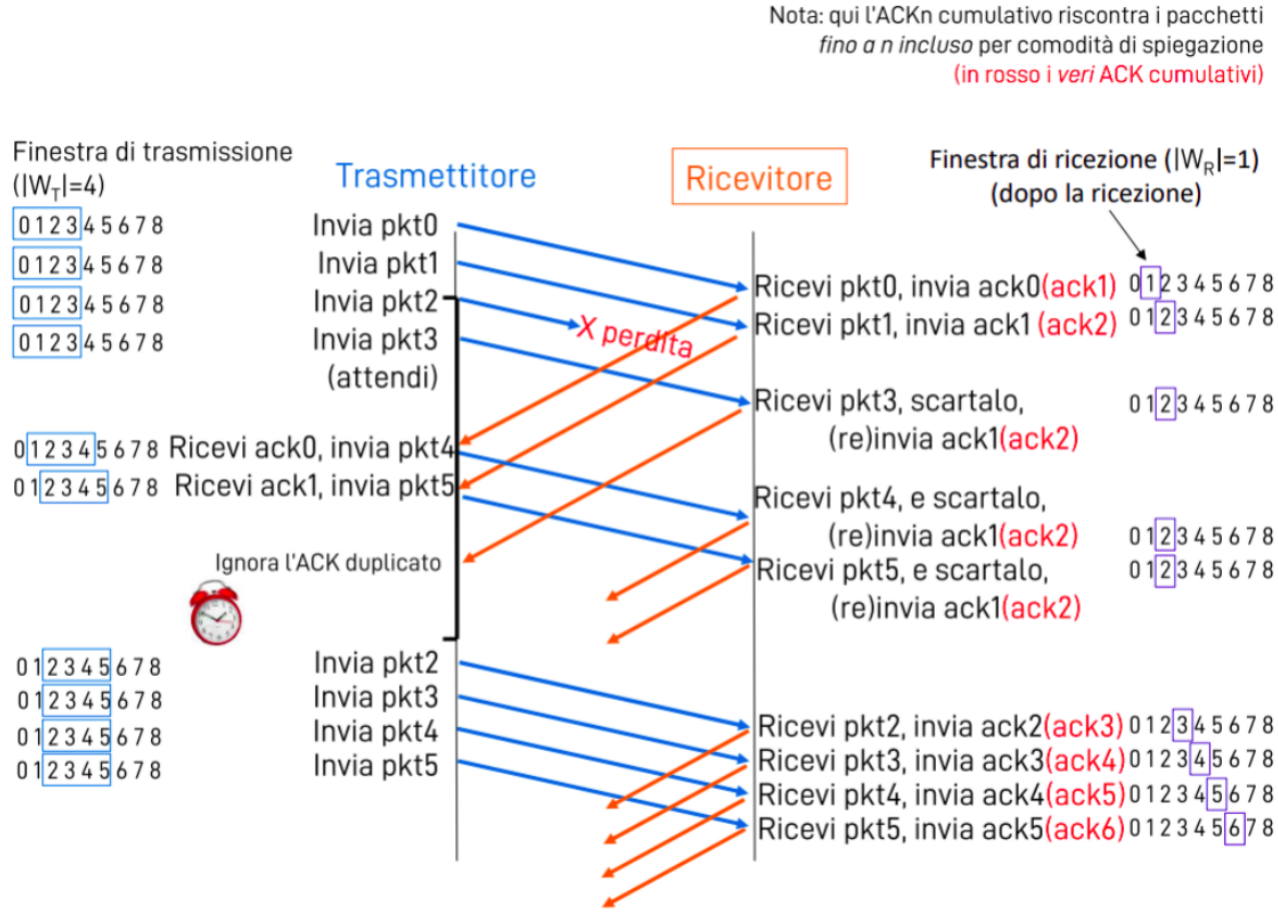
\includegraphics[width=\textwidth]{go-back-n.png}
    \caption{Funzionamento protocollo \emph{Go-back-N}}
\end{figure}\noindent
Ogni volta che il destinatario riceve un pacchetto e trasmette l'\emph{ACK},
quel pacchetto viene trasferito all'applicazione del ricevitore.

\subsection{Protocollo Selective repeat}
Come nel \emph{Go-back-N}, il mittente può avere fino a $N$ pacchetti senza
\emph{ACK}, ma diversamente da prima, il ricevente invia \emph{ACK individuali}.
Il mittente mantiene un timer per ciascun pacchetto non confermato e quando
scade ritrasmette il pacchetto associato a quel timer.

Un'altra differenza col \emph{Go-back-N} è che nel \emph{Selective repeat},
quando viene ricevuto un pacchetto successivo ad un pacchetto mancante, non
viene scartato, ma viene salvato in un buffer.

\begin{figure}[ht]
    \centering
    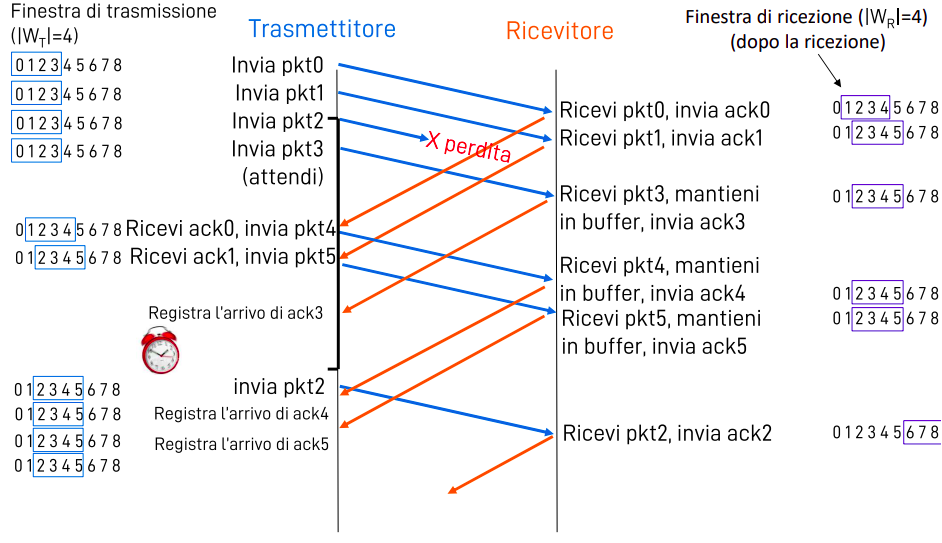
\includegraphics[width=\textwidth]{selective-repeat.png}
    \caption{Funzionamento protocollo \emph{Selective repeat}}
\end{figure}
\bigskip\noindent
Come prima, i pacchetti vengono consegnati all'applicazione del ricevitore ogni
volta che l'\emph{ACK} ad essi associato viene trasmesso. Nel caso di pacchetti
persi, quando questi vengono ricevuti, vengono inviati all'applicazione ricevente
il pacchetto appena arrivato e tutti quelli successivi che erano stati salvati
nel buffer.

\paragraph{Relazione tra numeri dimensione della finestra e numeri di sequenza}
Nel protocollo \emph{Selective repeat}, il numero di sequenza dei pacchetti è
ciclico, cioè, se vengono usati $k$ bit per codificare il numero di sequenza,
si avrà un periodo, ovvero una quantità di numeri di sequenza, pari a $2^k$.

Fissato $k$, la dimensione totale delle \emph{finestre di trasmissione} e
\emph{ricezione} deve esser minore o uguale a $2^k$, ovvero deve valere:
\[W_T+W_R\leq2^k\]
Nel caso particolare in cui $W_T=W_R$ deve valere:
\[W_T\leq2^{k-1}=\frac{2^k}{2}\]
Il motivo per il quale deve sussistere questa condizione è che, in questo modo,
i numeri di sequenza delle \emph{finestre di trasmissione} e di \emph{ricezione}
non potranno mai sovrapporsi. La sovrapposizione va evitata perché altrimenti
potrebbe accadere che il ricevente riconosca come pacchetti nuovi pacchetti che
in realtà sono già stati ricevuti.
\paragraph{Esempio di sovrapposizione}
In questo esempio, i numeri di sequenza sono codificati su 2 bit e le
\emph{finestre} hanno entrambe dimensione $3$, per cui $W_T+W_R=6>2^2=4$.

Vengono inviati e correttamente ricevuti i primi tre pacchetti. Di conseguenza,
la \emph{finestra di ricezione} viene shiftata tre volte e, alla fine, rimane
in attesa dei pacchetti con numeri $3$, $0$ e $1$. Tuttavia, se accade che
tutti e tre gli \emph{acknowledgement} vengono persi durante la trasmissione, il
mittente, non ricevendo nessuna conferma di ricezione, provvede ad impostare un
timer per ciascuno di essi.

Allo scadere del primo timer, il mittente ritrasmette il pacchetto con numero di
sequenza $0$ nella \emph{finestra di trasmissione}. Il destinatario lo riceve e,
poiché nella sua \emph{finestra di ricezione} è presente un pacchetto con numero
$0$, accetta il pacchetto ricevuto e trasmette un \emph{ACK}. Il problema è che
quel pacchetto in realtà era già stato ricevuto, quindi il ricevente si è
ritrovato con un pacchetto duplicato.

\begin{figure}[ht]
    \centering
    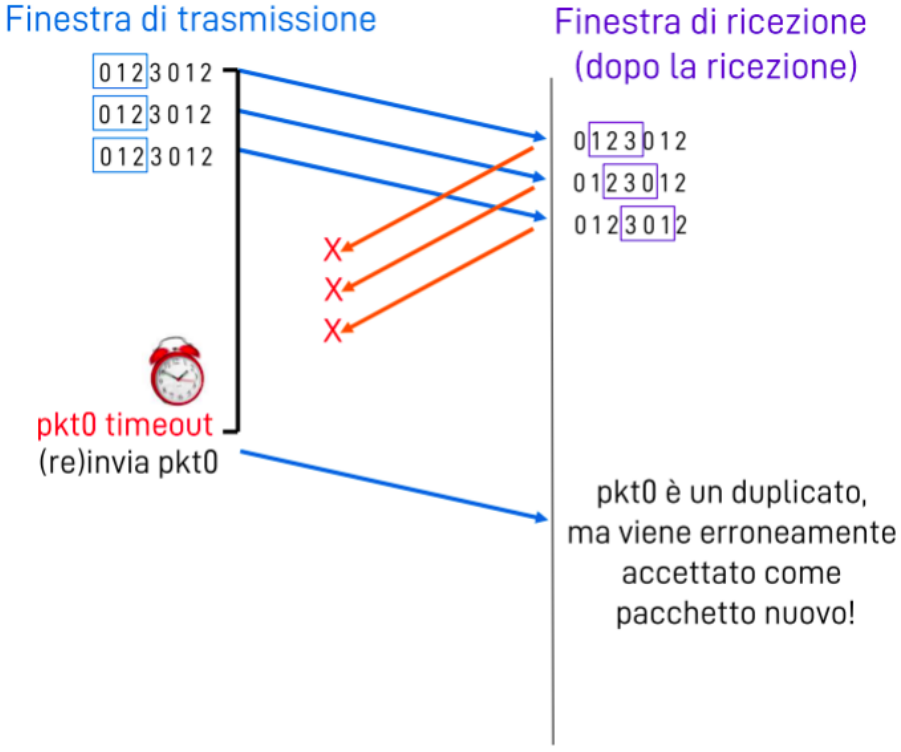
\includegraphics[width=0.8\textwidth]{selective-repeat-problema-num-seq.png}
    \caption{Esempio sovrapposizione numeri di sequenza nel \emph{Selective repeat}}
\end{figure}

\begin{note}
    Nel protocollo \emph{Go-back-N}, la condizione sui numeri di sequenza e sulle
    dimensioni delle finestre non vale, in quanto, il ricevente trasmette
    \emph{ACK cumulativi} e non shifta la \emph{finestra di ricezione} finché non
    riceve una sequenza completa di pacchetti.
    Di conseguenza, se i numeri di sequenza fossero codificati su $k$ bit e la
    \emph{finestra di trasmissione} avesse dimensione $2^k-1$, nell'ipotesi in
    cui tutti i pacchetti trasmessi venissero ricevuti, ma andassero persi tutti
    gli \emph{ACK}, se anche il mittente ritrasmettesse un pacchetto già
    ricevuto dal destinatario, questo lo scarterebbe poiché nella sua
    \emph{finestra di ricezione} quel numero di sequenza non ci sarebbe più.
\end{note}

\section{Protocollo TCP}
Il protocollo \emph{\gls{prot:TCP}} è un protocollo connesso che consente a due
\emph{host} di scambiarsi \emph{segmenti} in modo affidabile e ordinato. In
particolare, i \emph{segmenti TCP} viaggiano all'interno di una connessione
\emph{full duplex} che consente trasmissioni in entrambe le direzioni.

Il \emph{TCP} fa uso del \emph{pipelining}, quindi esistono \emph{finestre di
trasmissione e ricezione} la cui dimensione viene stabilita in base a meccanismi
di \emph{controllo di flusso} e \emph{congestione} e quindi varia nel tempo.

\paragraph{Struttura dei segmenti TCP}
Proprio per le garanzie offerte dal \emph{TCP}, la struttura dei \emph{segmenti}
è più complicata rispetto a quanto visto con i \emph{segmenti UDP}.

\begin{figure}[ht]
    \centering
    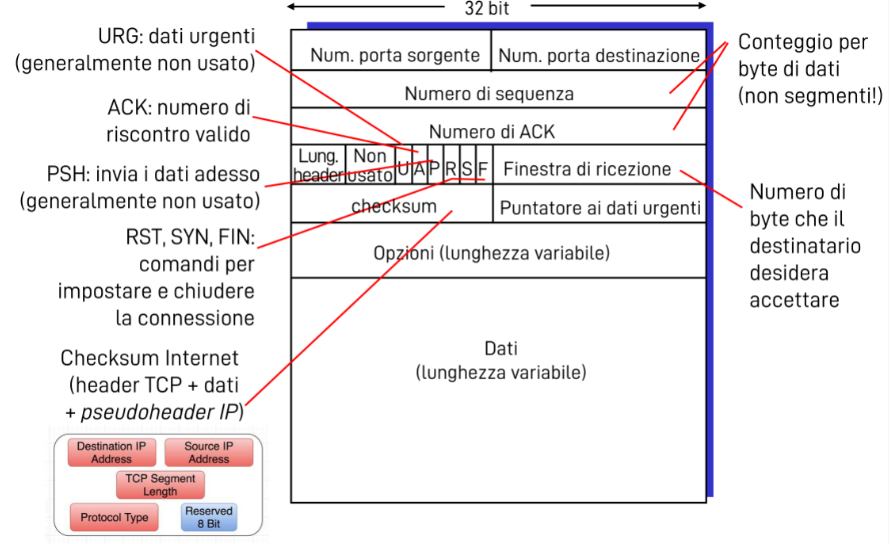
\includegraphics[width=0.75\textwidth]{struttura-messaggi-tcp.png}
    \caption{Struttura di un \emph{segmento TCP}}
\end{figure}
La dimensione della \emph{finestra di ricezione} indicata nel campo
\emph{\gls{glos:RWND}}\footnote{Nella figura si fa riferimento al campo
\texttt{Finestra di ricezione}}, è rappresentata da un valore a 16 bit,
che definisce il numero di byte che il destinatario può memorizzare. Di
conseguenza, rappresenta anche la massima quantità di dati che può essere
in transito durante un \emph{RTT}.

\noindent
Poiché \emph{RWND} è un valore a 16 bit, possono transitare contemporaneamente
$64kByte$. Tuttavia, è possibile aumentare quel limite usando un meccanismo di
\emph{scalatura}, cioè decidendo che quel valore non rappresenta il numero di
byte, ma un loro multiplo.

I campi \texttt{numero di sequenza} e \texttt{numero di ACK} indicano
rispettivamente il numero del primo byte di quel segmento all'intero del
\emph{flusso di dati} e il numero di sequenza del prossimo byte atteso dall'altro
lato, ricordando che il \emph{TCP} utilizza \emph{ACK cumulativi}.

\begin{note}
    Per quanto riguarda la gestione dei \emph{segmenti} fuori sequenza, il
    \emph{TCP} non stabilisce una policy unica, ma dipende dall'implementazione.
\end{note}

\begin{figure}[h!]
    \centering
    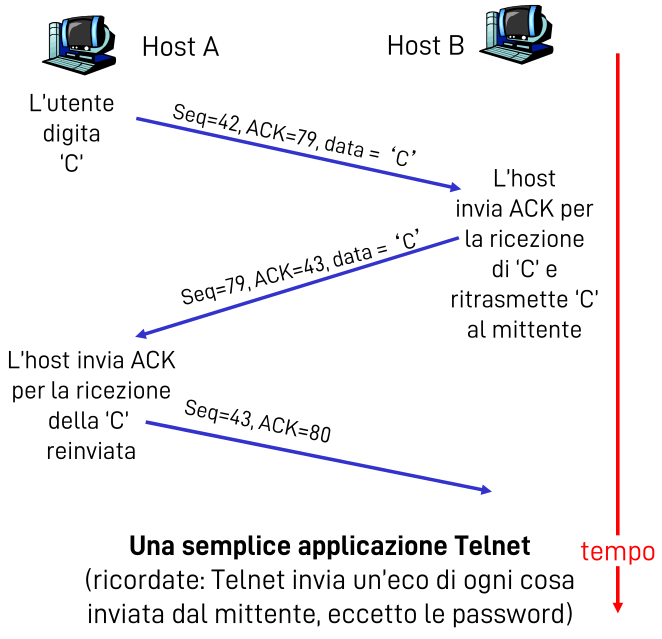
\includegraphics[width=0.55\textwidth]{tcp-esempio-telnet.png}
    \caption{\emph{Numeri di sequenza} e \emph{ACK} in una comunicazione \emph{TCP}}
\end{figure}

\subsection{Instaurazione di una connessione TCP}
Una connessione \emph{TCP} viene instaurata mediante un meccanismo detto
\emph{Three-way handshake}:
\begin{enumerate}
    \item L'\emph{host A} inizia la connessione, quindi, invia all'\emph{host B}
    un \emph{segmento} con flag \texttt{SYN} impostato a $1$, porta sorgente pari
    ad $A$, porta destinazione $B$ e numero di sequenza iniziale $x$;
    \item L'\emph{host B} riceve il \emph{segmento} di inizializzazione e risponde
    con un \emph{segmento} nel quale i flag \texttt{SYN} e \texttt{ACK} sono
    impostati a $1$, le porte sorgente e destinazione sono rispettivamente $B$
    ed $A$, il numero di sequenza iniziale è $y$ e il numero di \emph{ACK} $x+1$;
    \item L'\emph{host A} risponde inviano un \emph{segmento ACK} con porta
    sorgente $A$, destinazione $B$ e numero di \emph{ACK} $y+1$;
\end{enumerate}
\begin{figure}[h!]
    \centering
    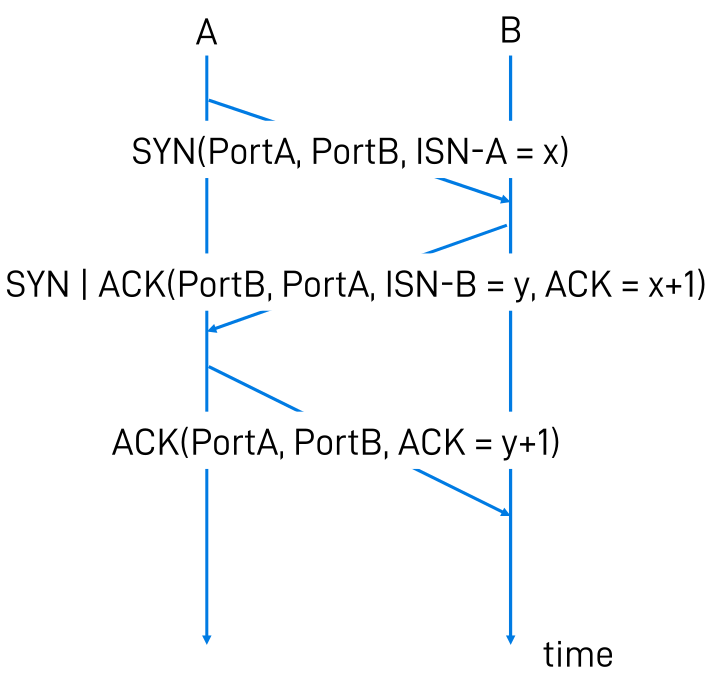
\includegraphics[width=0.6\textwidth]{tcp-three-way-handshake.png}
    \caption{Meccanismo di \emph{Three-way handshake} nel \emph{TCP}}
\end{figure}
\begin{note}
    \emph{ISN} sta per \emph{Initial Sequence Number} ed è il numero di
    partenza dei numeri di sequenza che non iniziano necessariamente da
    zero.
\end{note}

\subsection{Dimensione dei segmenti}
Sebbene il protocollo \emph{TCP} gestisca i dati organizzandoli byte, non invia
mai singoli byte, ma cerca di accorparli in un unico \emph{segmento} di dimensione
massima\footnote{Il \emph{TCP} può essere costretto ad inviare singoli byte}.

L'\emph{\gls{glos:MSS}} dipende da un parametro del \emph{livello} sottostante,
il \emph{livello Rete}, che si chiama \emph{\gls{glos:MTU}}, il quale a sua
volta dipende dall'\emph{MTU} del \emph{livello Data Link}. Tutti questi parametri
dipendono anche dalle specifiche dei collegamenti attraverso i quali dovranno
transitare i dati.

Comunque, l'\emph{MSS} indica la dimensione massima del \emph{payload}, cioè i
dati trasportati dal \emph{segmento}. Tuttavia, poiché non esistono meccanismi
per la negoziazione di questo parametro, il \emph{TCP} procede per
tentativi, andando progressivamente ad incrementarlo fino a quando non viene
perso qualche \emph{segmento} o non viene ricevuta una comunicazione esplicita di
incompatibilità\footnote{Non viene inviata sempre, dipende dalla configurazione
dei singoli \emph{host}}.

Di default, l'\emph{MSS} viene impostata a 1460 byte (1500 byte per l'\emph{MTU}
del \emph{livello Data Link} e 40 byte per gli \emph{header TCP} e \emph{IP}).

In ogni caso, esiste una dimensione minima fissata a 536 byte dovuta al fatto
che il protocollo \emph{\gls{prot:IP}} richiede una \emph{MTU} minima
di 576 byte (536 byte per il \emph{payload} e 40 byte di \emph{header}).

\subsection{Chiusura di una connessione TCP}
Poiché le connessioni \emph{TCP} sono bidirezionali, al termine della comunicazione,
vanno chiuse in entrambe le direzioni. Esistono due modalità di terminazione:
una cosiddetta \quotes{gentile} e una \quotes{brusca}.

\paragraph{Modalità \quotes{gentile}}
L'\emph{host} che intende terminare la connessione invia un \emph{segmento} nel
quale il flag \texttt{FIN} è impostato a 1 e il ricevitore risponde con un \emph{ACK}.
A questo punto la connessione è chiusa per metà, in quanto il primo \emph{host}
non può più trasmettere nulla, ad eccezione degli \emph{acknowledgement}, mentre
il secondo può continuare ad inviare \emph{segmenti}.

Per terminare del tutto la connessione è necessario che anche il secondo
\emph{host} invii un \emph{segmento} con flag \texttt{FIN} a 1.

\begin{figure}[h!]
    \centering
    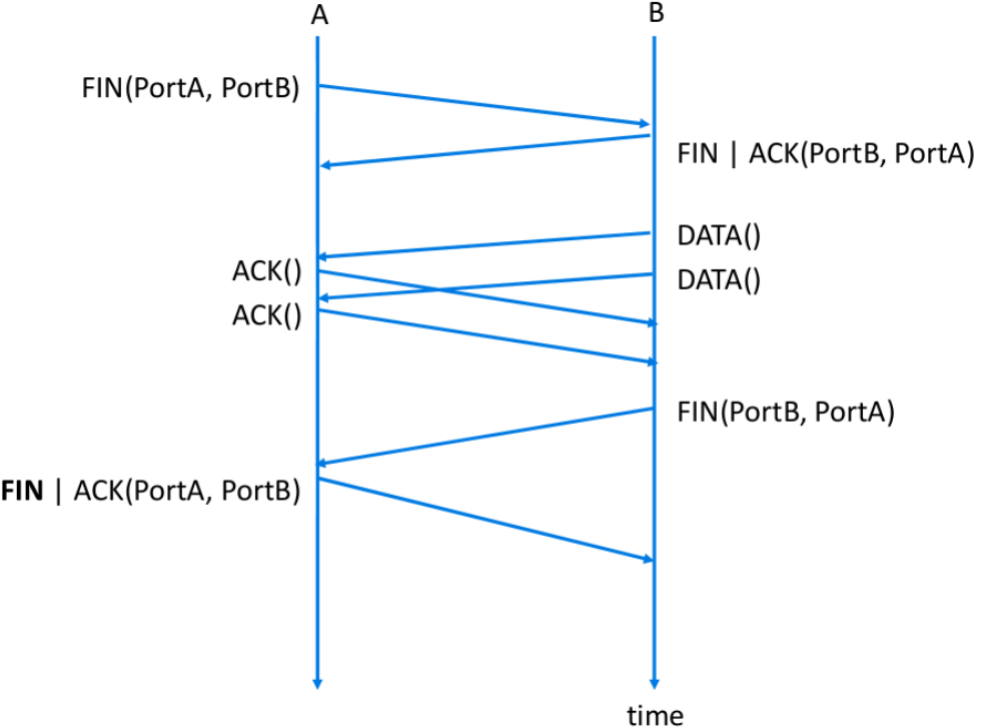
\includegraphics[width=0.8\textwidth]{tcp-chiusura-gentile.png}
    \caption{Chiusura \quotes{gentile} di una connessione \emph{TCP}}
\end{figure}

\paragraph{Modalità \quotes{brusca}}
Questa modalità viene usata per resettare connessioni non più gestibili o
che si trovano in uno stato di errore (e.g. viene ricevuto un \emph{ACK} su una
connessione mai aperta). Per farlo, uno degli \emph{host} invia un
\emph{segmento} con flag \texttt{RST} impostato a 1. Quindi, entrambi gli
\emph{host} liberano le risorse allocate dal sistema operativo per quella
connessione.

\begin{note}
    I server possono usare questa tecnica per chiudere velocemente le
    connessioni con i client.
\end{note}

\begin{figure}[ht]
    \centering
    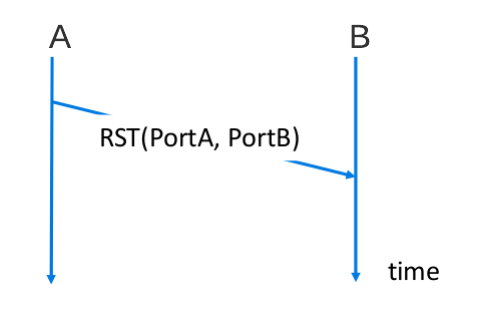
\includegraphics[width=0.4\textwidth]{tcp-chiusura-brusca.png}
    \caption{Chiusura \quotes{brusca} di una connessione \emph{TCP}}
\end{figure}

\subsection{Stimare l'RTT e scegliere l'RTO}
La scelta dell'\emph{\gls{glos:RTO}}, ovvero la durate dei timer, influenza le
prestazioni della comunicazione. Se viene scelto un valore troppo piccolo, c'è
il rischio vengano effettuate delle ritrasmissioni non necessarie, mentre al
contrario, un valore troppo grande rende il \emph{TCP} troppo poco reattivo
alle perdite. In ogni caso, l'\emph{RTO} deve essere maggiore
dell'\emph{\gls{glos:RTT}}, che però è soggetto a variazioni.

\begin{definition}[SampleRTT]
    Il sampleRTT è il tempo misurato dalla trasmissione di un segmento alla
    ricezione del relativo ACK, ignorando le ritrasmissioni.
\end{definition}\noindent
Poiché il \emph{sampleRTT} è diverso per ogni \emph{segmento}, viene realizzata
una stima partendo dalla media dei precedenti valori di \emph{sampleRTT}\footnotemark.
\footnotetext{Si effettua una media pesata che da maggiore peso ai valori più
recenti e progressivamente meno peso a quelli più vecchi.}
Il tempo stimato viene calcolato, partendo dalla stima precedente, mediante una
\emph{media mobile esponenziale ponderata} e, in particolare, vale la seguente
formula:
\[\emph{EstimatedRTT}=(1-\alpha)\cdot\emph{EstimatedRTT}+\alpha\cdot
\emph{SampleRTT}\quad\text{per }\alpha=0.125\]
Con questo tipo di formula, il peso dei campioni precedenti diminuisce
esponenzialmente.

A questo punto, l'\emph{RTO} può essere definito pari alla stima dell'\emph{RTT}
con in aggiunta un margine di sicurezza. Per fare ciò, bisogna innanzitutto
sapere di quanto il valore stimato per l'\emph{RTT} si discosta da quello reale:
\[\emph{DevRTT}=(1-\beta)\cdot\emph{DevRTT}+\beta\cdot|\emph{SampleRTT}-
\emph{EstimatedRTT}\,|\quad\text{per }\beta=0.25\]
Anche in questo caso, la deviazione viene calcolata a partire dal valore precedente.
Il \emph{DevRTT} costituisce il valore di partenza per la definizione del margine
di sicurezza. Noto ciò, l'\emph{RTO} è definito come:
\[\emph{RTO}=\emph{EstimatedRTT}+4\emph{DevRTT}\]

\begin{figure}[ht]
    \centering
    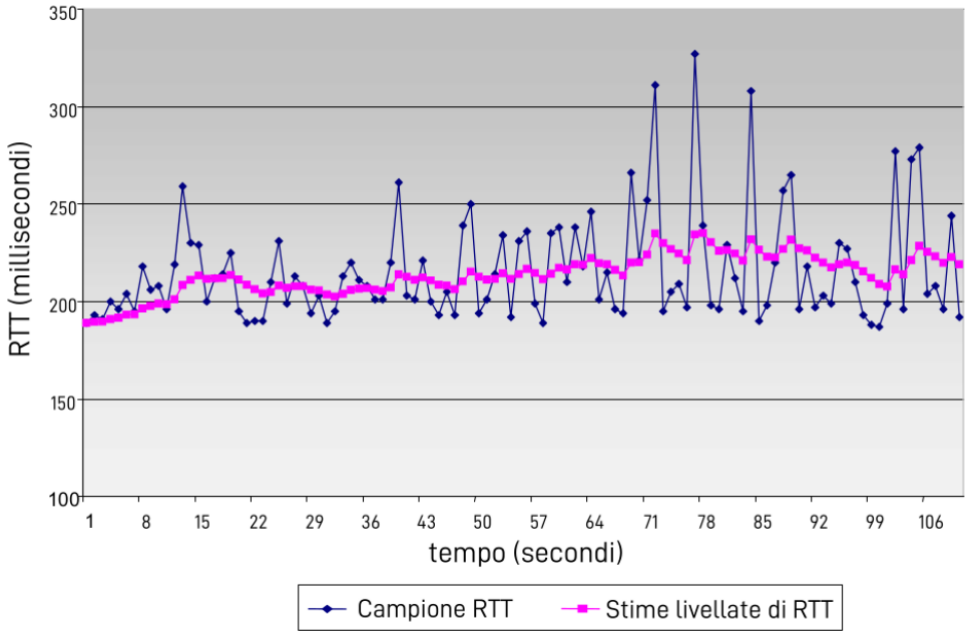
\includegraphics[width=0.8\textwidth]{tcp-stima-rtt.png}
    \caption{Confronto tra \emph{RTT} reale e stimato}
\end{figure}

\paragraph{Inizializzazione dei valori}
Ovviamente, all'avvio della comunicazione \emph{EstimatedRTT} e \emph{DevRTT}
non sono definiti, quindi devono essere inizializzati a un qualche valore. Lo
standard stabilisce che quando si è in possesso di una sola misura di \emph{RTT},
si pongono $\emph{EstimatedRTT}=\emph{SampleRTT}$ e $\emph{DevRTT}=\emph{SampleRTT}/2$.
L'\emph{RTO} viene invece inizializzato a un secondo. Col procedere della
comunicazione i valori verranno progressivamente affinati.

\subsection{Controllo di flusso}
Il \emph{\nameref{def:7}}, come già accennato, è una delle funzionalità
offerte dal protocollo \emph{TCP} e permette al ricevitore di controllare la
velocità di trasmissione del mittente in modo da evitare di sovraccaricarsi.

Per farlo, il ricevitore comunica al mittente la quantità di spazio ancora
disponibile nel proprio buffer di ricezione e lo fa, indicando nell'\emph{header}
di ogni \emph{segmento} il valore della \emph{RWND}. Il mittente, quindi, limita
la propria \emph{finestra di trasmissione} al valore indicatogli dal ricevente.

Questa scelta garantisce che il buffer del destinatario non andrà mai in
overflow costringendolo a scartare i \emph{segmenti} ricevuti per mancanza di
spazio.

\begin{figure}[h!]
    \centering
    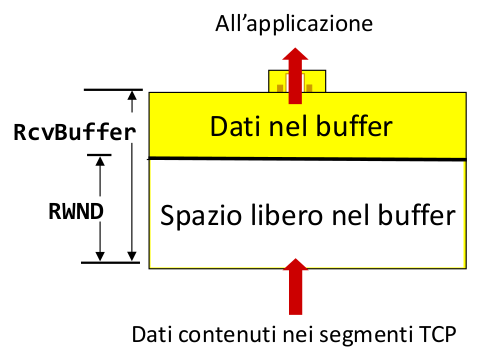
\includegraphics[width=0.5\textwidth]{buffering-al-ricevitore-tcp.png}
    \caption{Gestione del buffer di ricezione}
\end{figure}
\newpage
\begin{figure}[ht!]
    \centering
    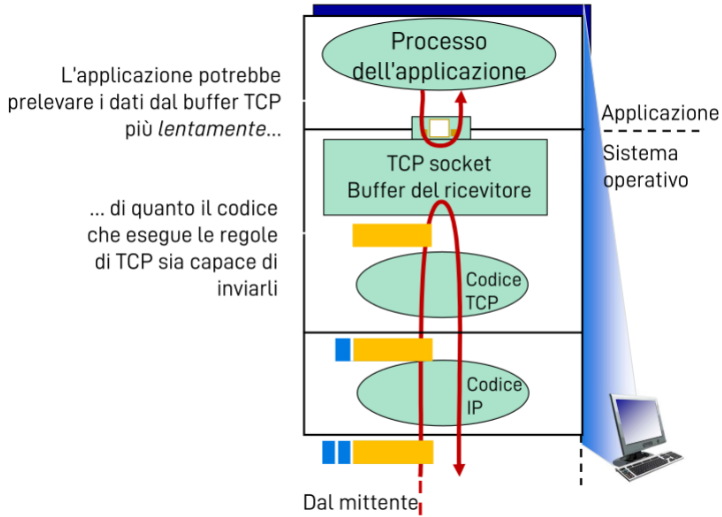
\includegraphics[width=0.6\textwidth]{controllo-flusso-tcp.png}
    \caption{Gestione dello \emph{stack protocollare} al ricevitore}
\end{figure}

\section{Gestione della congestione}
Abbiamo già dato una definizione di \nameref{def:6}, ma informalmente possiamo
dire che la \emph{congestione} si verifica quando troppi trasmettitori stanno
inviando troppi dati e la rete non è in grado di gestire tutto quel traffico.
Una rete congestionata comporta la perdita di \emph{pacchetti}, dovuta
all'overflow dei buffer nei \emph{router}, e lunghi ritardi nel trasferimento,
dovuti all'accodamento dei \emph{pacchetti} nei buffer.

\subsection{Modelli per sistemi a coda}
Un \emph{sistema a coda} comprende una \quotes{fila d'attesa}, realizzata
solitamente con una \emph{coda}, e un \emph{server}. I parametri presi in
considerazione sono due:
\begin{enumerate}
    \item \emph{Tasso di arrivo $\lambda$}: è il numero medio di \emph{pacchetti},
    o in generale di \emph{unità di lavoro}, che entrano nella \emph{coda} per
    unità di tempo;
    \item \emph{Tasso di servizio $\mu$}: è il tempo medio richiesto dal
    \emph{server} per trasmettere un \emph{pacchetto}, o in generale per concludere
    un lavoro;
\end{enumerate}\noindent
Gli \emph{arrivi} e i \emph{tempi di servizio} sono distribuiti secondo
distribuzioni statistiche. Ad esempio, nei \emph{sistemi a coda} di tipo
$M/M/1$\footnotemark, gli \emph{arrivi} sono distribuiti come $exp\left(\frac{1}
{\lambda}\right)$, i \emph{tempi di servizio} come $exp\left(\frac{1}{\mu}\right)$
e c'è un solo \emph{server} a ricevere i \emph{pacchetti}.
\footnotetext{$M$ sta per \emph{Markovian} e si riferisce alla distribuzione
esponenziale.}

\begin{figure}[h!]
    \centering
    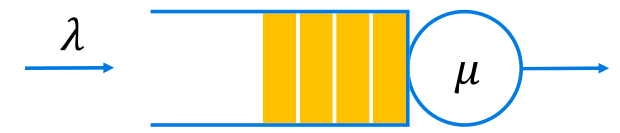
\includegraphics[width=0.8\textwidth]{sistemi-a-coda.png}
    \caption{Schema di un \emph{sistema a coda}}
\end{figure}\noindent
Le proprietà dei \emph{sistemi a coda} possono essere calcolate analiticamente.
Ad esempio, nei \emph{sistemi} $M/M/1$ si ha che:
\begin{itemize}
    \item \emph{Carico del server}: $\rho=\frac{\lambda}{\mu}$;
    \item \emph{Lunghezza media della coda}: $L=\frac{\rho^2}{1-\rho}$ per $\rho<1$;
    \item \emph{Probabilità che in un qualunque momento ci siano $n$ pacchetti in
    coda}: $\pi_n=(1-\rho)\cdot\rho^n$;
\end{itemize}
Poiché $\lambda$ e $\mu$ sono medie statistiche e non delle costanti, i dati
reali non coincidono sempre con quelli stimati. Inoltre, la probabilità che i
\emph{pacchetti} si accodino, anche se molto piccola, non è mai nulla.

\subsection{Cause della congestione}
Vediamo ora come si manifesta la \emph{congestione} in alcuni scenari.
\paragraph{Scenario 1}
Si supponga di avere due trasmettitori e due ricevitori e che i dati debbano
passare per un \emph{router} con un buffer infinito. Se la \hyperlink{sym:2}
{\emph{capacità del link}} di uscita è $R$ e non ci sono ritrasmissioni, il
\emph{throughput} massimo è $\frac{R}{2}$. Inoltre, se il \emph{tasso}
$\lambda_{in}$ si avvicina a $\frac{R}{2}$ si avrà a che fare con lunghi ritardi.

\begin{figure}[h!]
    \centering
    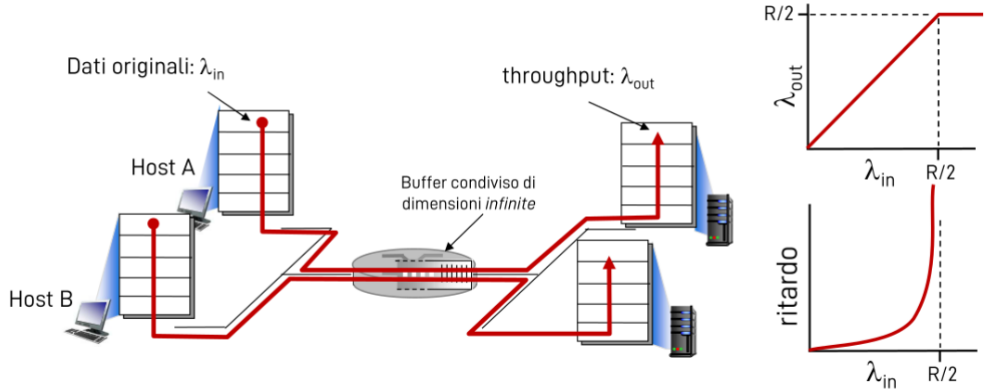
\includegraphics[width=0.8\textwidth]{congestione-scenario-1.png}
    \caption{\emph{Congestione} - scenario 1}
\end{figure}

\paragraph{Scenario 2}
Si supponga di avere un \emph{router} con un buffer di dimensione finita e che il
mittente ritrasmetta i pacchetti finiti in timeout. Si indichi con $\lambda_{in}$
il \emph{tasso di arrivo} dall'applicazione al mittente e con $\lambda_{out}$
il \emph{tasso} percepito dall'applicazione del destinatario.

Poiché il mittente ritrasmette i pacchetti persi, vengono inviati più dati di
quelli che si invierebbero se non ci fossero ritrasmissioni, di conseguenza se si
calcola il \emph{tasso di arrivo} al \emph{livello Trasporto}, e lo si indica con
$\lambda'_{in}$, si ha che $\lambda'_{in}>\lambda_{in}$, in quanto il \emph{livello
Trasporto} include anche tutte le ritrasmissioni.

In questo scenario possiamo distinguere due casi:
\begin{itemize}
    \item \emph{Caso ideale}: si ha una perfetta conoscenza della situazione e
    quindi il mittente può inviare dati solo quando sa che nel buffer del
    \emph{router} c'è spazio per riceverli;
    \item \emph{Caso realistico}: si ha una conoscenza limitata della rete e
    quando scatta un timeout, il mittente ritrasmette il \emph{pacchetto}
    associato, ma potrebbe accadere che vengano consegnate entrambe le copie
    causando un dimezzamento del \emph{throughput};
\end{itemize}\noindent
Nel \emph{caso realistico} è possibile ipotizzare cosa accadrebbe se il mittente
ritrasmettesse i \emph{pacchetti} solo quando è sicuro che questi siano andati
persi, per esempio impostando timer piuttosto lunghi. In questo modo si potrebbe
migliorare il \emph{throughput}, tuttavia, è comunque possibile che a causa della
\emph{congestione} anche i pacchetti ritrasmessi vengano persi.
\begin{figure}[ht!]
    \centering
    \subfloat[\emph{Caso ideale}]{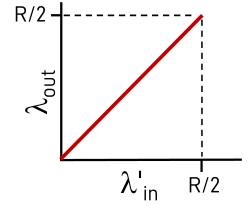
\includegraphics[width=0.3\textwidth]{congestione-scenario-2-caso-ideale.png}}
    \hfill
    \subfloat[\emph{Caso realistico}]{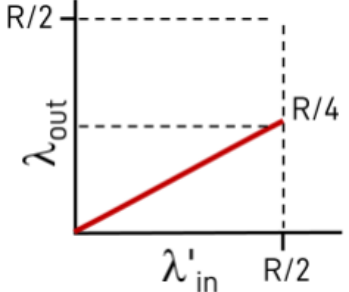
\includegraphics[width=0.3\textwidth]{congestione-scenario-2-caso-reale.png}}
    \hfill
    \subfloat[\emph{Caso realistico con certezza della perdita}]{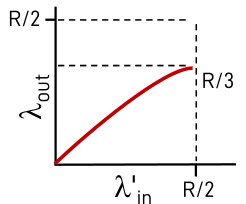
\includegraphics[width=0.3\textwidth]{congestione-scenario-2-caso-reale-idealizzato.png}}
    \caption{\emph{Congestione} - scenario 2}
\end{figure}

\paragraph{Scenario 3}
Si supponga che siano possibili più percorsi e che i \emph{pacchetti} debbano
passare attraverso più di un \emph{router}. Se accade che $\lambda'_{in}$ e
$\lambda_{in}$ aumentano, la maggior parte, se non tutti, i \emph{pacchetti}
trasmessi vengono scartati portando $\lambda_{out}$ a 0.

\begin{figure}[h!]
    \centering
    \subfloat[Schema dello scenario]{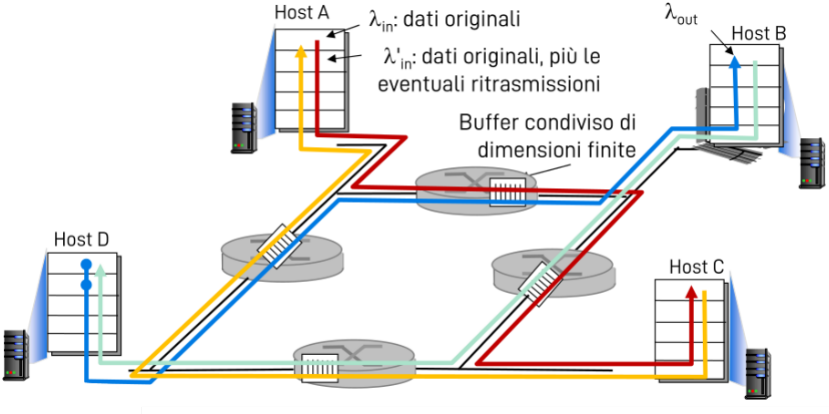
\includegraphics[width=0.7\textwidth]{congestione-scenario-3.png}}
    \hfill
    \subfloat[Grafico del ritardo]{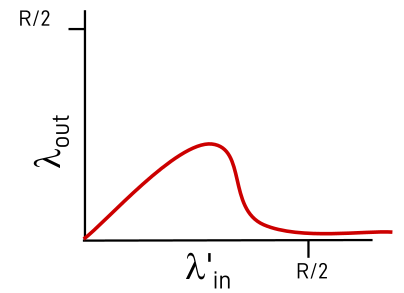
\includegraphics[width=0.28\textwidth]{congestione-scenario-3-grafico.png}}
    \caption{\emph{Congestione} - scenario 3}
\end{figure}

\begin{note}
    Ogni volta che un \emph{pacchetto} viene perso, tutte le risorse usate
    per portarlo fino a quel punto risultano sprecate.
\end{note}\noindent
In conclusione, possiamo affermare che con buffer infiniti non ci sono perdite, ma
se il \emph{tasso di invio} si avvicina troppo al \emph{tasso di servizio} i
ritardi si allungano di molto. Se i ritardi sono dovuti alla \emph{congestione}
provocata dalle ritrasmissioni fatte al termine di un timeout, si ha uno spreco
di risorse per via di ritrasmissioni inutili. Infine, se la \emph{congestione}
porta alla perdita dei \emph{pacchetti} si è costretti a pagare il costo della
loro ritrasmissione e lo sforzo richiesto per ridurre il tempo $\lambda'_{in}$
può provocare un crollo del \emph{throughput} vanificando così gli sforzi fatti.

\section{Controllo della congestione in TCP}
Il \emph{TCP} usa tecniche di \emph{controllo della congestione} per adattare
il \emph{tasso di trasmissione} alle condizioni della rete ed evitare di
congestionarla. Per fare ciò esistono diversi approcci:
\begin{itemize}
    \item \emph{Controllo di congestione end-to-end}: il livello di
    \emph{congestione} viene stimato tenendo traccia dei \emph{segmenti} persi
    e dei ritardi;
    \item \emph{Controllo di congestione assistito dalla rete}: i \emph{router}
    forniscono dei feedback agli \emph{host} sullo stato della rete
    (e.g. viene impostato un bit per indicare la \emph{congestione});
\end{itemize}
Non esiste un unico protocollo per il \emph{controllo della congestione}, ma
implementazioni diverse del \emph{TCP} adottano soluzione distinte.

\subsection{Protocollo AIMD}
Nel protocollo \emph{\gls{prot:AIMD}} il mittente aumenta progressivamente il
\emph{tasso di trasmissione}, cosa che coincide con l'aumento della dimensione
della \emph{finestra di trasmissione}, cercando di occupare tutta la banda
disponibile. Quando viene rilevata una perdita, la dimensione della \emph{finestra}
viene ridotta.

\bigskip\noindent
Questo protocollo è organizzato in due fasi:
\begin{itemize}
    \item \emph{Additive increase}: ad ogni \emph{\gls{glos:RTT}}, fino a quando
    non viene rilevata una perdita, la \emph{finestra di trasmissione} viene
    aumentata di una \emph{\gls{glos:MSS}};
    \item \emph{Multiplicative decrease}: quando viene rilevata una perdita, la
    \emph{finestra di trasmissione} viene dimezzata;
\end{itemize}

\begin{figure}[h!]
    \centering
    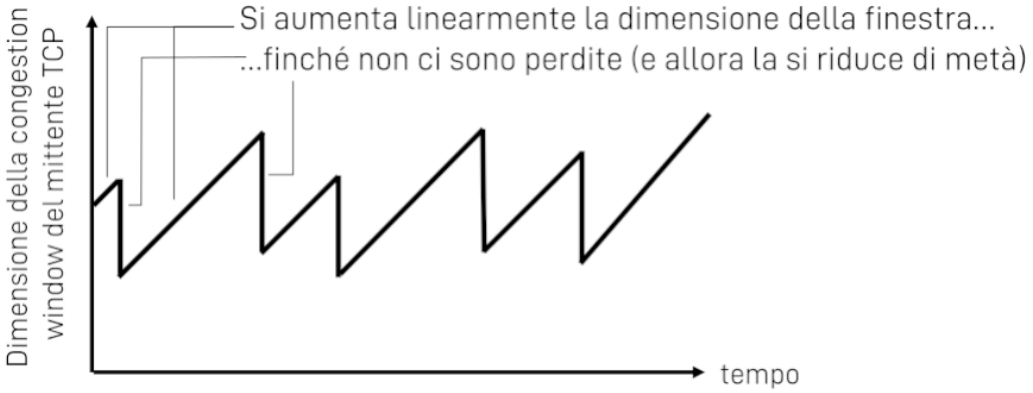
\includegraphics[width=0.9\textwidth]{tcp-aimd.png}
    \caption{Dimensione della \emph{finestra di trasmissione} in funzione del tempo}
\end{figure}

\begin{note}
    In realtà, più che di \emph{finestra di trasmissione} sarebbe meglio parlare
    di \emph{finestra di congestione}.
\end{note}
\begin{definition}[Finestra di congestione]
    La finestra di congestione è l'insieme delle PDU che possono essere
    inviate nella rete e la sua dimensione è definita in base alla quantità
    massima di dati che il mittente pensa di poter inviare senza sovraccaricare
    la rete.
\end{definition}\noindent
La dimensione della \emph{\gls{glos:CWND}} è soggetta a variazioni durante la
comunicazioni in quanto il valore viene deciso dinamicamente dall'algoritmo di
\emph{controllo della congestione}. Un'altra cosa che cambia durante la
comunicazione è la \emph{finestra di trasmissione}.

\begin{definition}[Finestra di trasmissione]
    La finestra di trasmissione è l'insieme delle PDU che possono essere inviate
    in rete senza saturare il ricevitore e la sua dimensione è definita come:
    \[|W_T|=\min(\emph{CWND},\,\emph{RWND})=\min(\emph{CWND},\,|W_R|)\]
\end{definition}

\paragraph{Fairness}
Il protocollo \emph{AIMD} permette di ottenere una distribuzione equa delle
risorse di rete. Ciò significa che se $k$ sessioni \emph{TCP} si dividono lo
stesso collegamento di banda $R$ che fa da collo di bottiglia, ogni sessione
dovrebbe percepire la stessa banda $\frac{R}{k}$. Questa caratteristica è
detta \emph{fairness}.

Ad esempio, se due connessioni stanno condividendo lo stesso collegamento,
nel corso del tempo, il processo di \emph{additive increase} fa aumentare la
\emph{banda} di entrambe le connessioni in modo lineare. D'altra parte, quando
si passa alla fase di \emph{multiplicative decrease}, la \emph{banda} viene
ridotta in modo proporzionale a quella che si stava utilizzando. Ciò significa
che la diminuzione sarà maggiore per la connessione che stava occupando la
fetta maggiore di \emph{banda}.

\begin{figure}[h!]
    \centering
    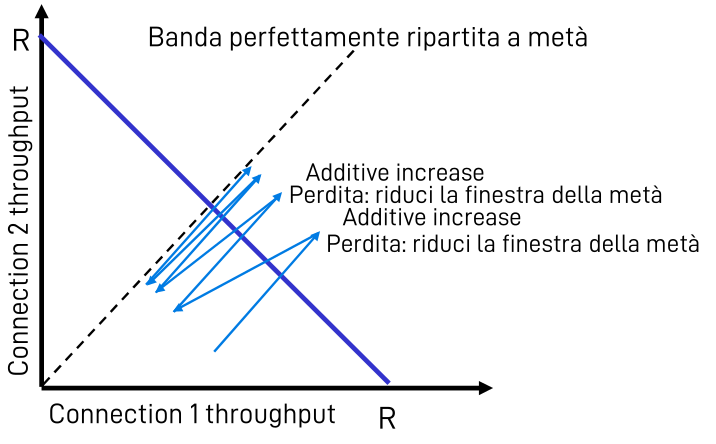
\includegraphics[width=0.7\textwidth]{tcp-aimd-fairness.png}
    \caption{Raggiungimento dello stato di \emph{fairness}}
\end{figure}

\paragraph{Slow Start e Congestion Avoidance}
L'algoritmo \emph{AIMD} suddivide la comunicazione in due fasi che si alternano:
\begin{itemize}
    \item \emph{Slow Start}: il mittente trasmette inizialmente un solo
    \emph{segmento} e, per ogni \emph{ACK} valido ricevuto, incrementa di una
    \emph{MSS} la \emph{CWND}, che quindi aumenta esponenzialmente la propria
    dimensione.

    Quando la \emph{CWND} raggiunge un valore soglia \emph{\gls{glos:SSTHRESH}}
    l'algoritmo passa in regime di \emph{Congestion Avoidance};
    \item \emph{Congestion Avoidance}: per ogni \emph{ACK} valido ricevuto, la
    \emph{CWND} aumenta di $MSS\cdot\frac{MSS}{CWND}$ byte ovvero $\frac{1}{CWND}$
    \emph{segmenti}. Ciò significa che per ogni \emph{RTT}, se vengono ricevuti
    tutti gli \emph{ACK} attesi (sono tanti quanto è la \emph{CWND}), la
    \emph{CWND} viene incrementata di una \emph{MSS} (un \emph{segmento}).
    In questa fase l'incremento della \emph{CWND} è lineare.
\end{itemize}

\begin{figure}[ht]
    \centering
    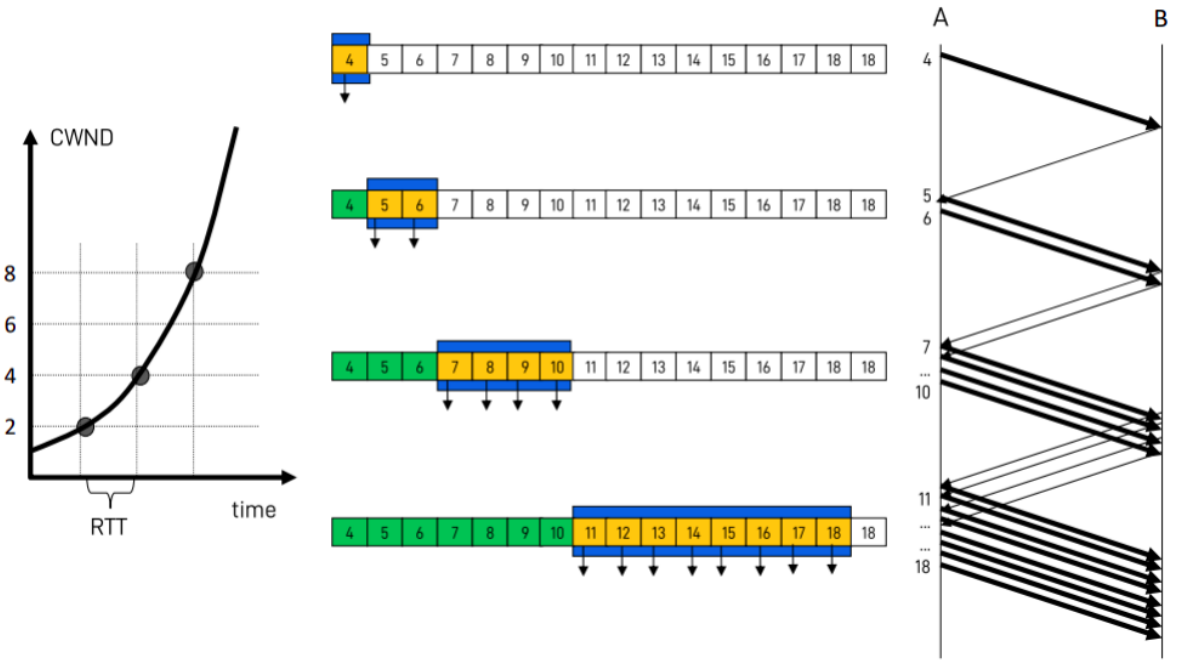
\includegraphics[width=\textwidth]{slow-start-ex.png}
    \caption{Crescita della \emph{CWND} in regime di \emph{slow start}}
\end{figure}
\newpage
\begin{figure}[h!]
    \centering
    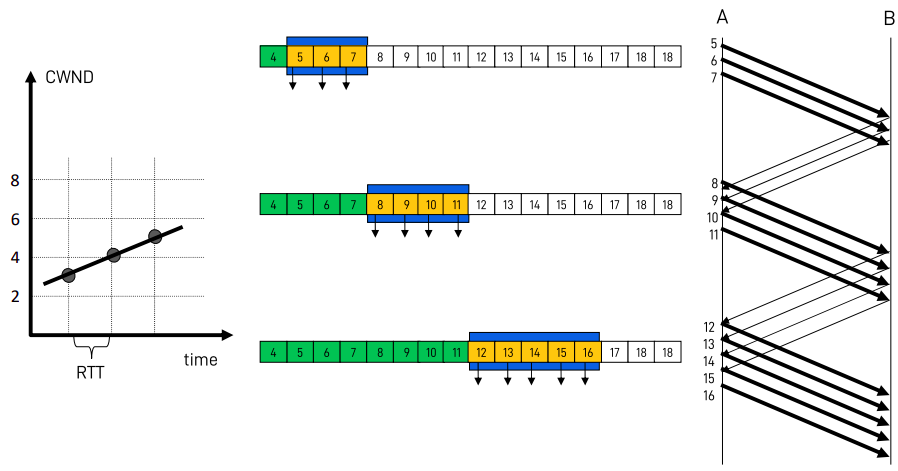
\includegraphics[width=\textwidth]{congestion-avoidance-ex.png}
    \caption{Crescita della \emph{CWND} in regime di \emph{congestion avoidance}}
\end{figure}\noindent
Lavorando con l'\emph{AIMD} è possibile modificare le prestazioni della
comunicazione andando ad agire su quattro parametri:
\begin{itemize}
    \item \emph{CWND}: è possibile aumentarla per trasmettere di più, ma ciò
    rende più probabile andare a congestionare la rete;
    \item \emph{SSTHRESH}: diminuendola si conclude riduce la fase di crescita
    esponenziale e si passa prima in \emph{congestion avoidance} favorendo
    un approccio più prudente;
    \item \emph{\emph{\gls{glos:RTO}}}: aumentandolo si aumenta il tempo di
    attesa di ciascun \emph{ACK};
    \item \emph{$W_{LOW}$ e $W_{UP}$}: è possibile ritardarne lo spostamento in
    modo, per esempio, di mantenere in memoria \emph{segmenti} per i quali non
    si è ancora ricevuto l'\emph{ACK};
\end{itemize}

\paragraph{Funzionamento dell'algoritmo}
L'algoritmo parte in regime di \emph{Slow Start} e inizializza la \emph{CWND}
e la \emph{SSTHRESH}, rispettivamente, a $1$ \emph{MSS} e a \emph{RWND}\footnote
{In alcune implementazioni viene impostata a $\frac{RWND}{2}$.}.
Essendo in \emph{Slow Start}, per ogni \emph{ACK} valido ricevuto la \emph{CWND}
viene incrementata di una \emph{MSS} e il puntatore $W_{LOW}$ viene spostato al
primo byte (o \emph{segmento}) non confermato.
Se $\emph{CWND}\geq\emph{SSTHRESH}$ l'algoritmo passa in \emph{Congestion
Avoidance}, altrimenti continua ad inviare \emph{pacchetti}.

Quando l'algoritmo si trova in regime di \emph{Congestion Avoidance},
per ogni \emph{ACK} valido ricevuto la \emph{CWND} viene incrementata di
$MSS\cdot\frac{MSS}{CWND}$ byte e il puntatore $W_{LOW}$ viene spostato al
primo \emph{segmento} non validato. Fatto ciò, vengono trasmessi altri
\emph{segmenti}.

\bigskip\noindent
In entrambe le fasi, quando per un \emph{segmento} non si riceve nessun
\emph{ACK}, ovvero quando scatta il timeout associato al \emph{segmento}, la
soglia di \emph{SSTHRESH} viene abbassata a $\max\left(\frac{CWND}{2}, 2\right)$,
viene raddoppiato l'\emph{RTO}, viene reimpostata ad $1$ \emph{MSS} la
\emph{CWND} e, quindi, viene ritrasmesso il \emph{segmento} perso.

\begin{note}
    L'utilizzo del solo \emph{RTO} non è efficiente in quanto costringe ad
    attendere lo scadere del timer prima di procedere con il rinvio.
\end{note}

\paragraph{Fast retransmit e fast recovery}
Un modo migliore di gestire le perdite può essere realizzato sfruttando la
natura degli \emph{ACK}, che in \emph{TCP} sono \emph{cumulativi}. In particolare,
quando viene perso un \emph{segmento}, alla ricezione dei successivi, il destinatario
non risponde con gli \emph{ACK} corrispondenti, ma ripropone l'ultimo \emph{ACK}
mandato prima della perdita.

Quindi, il mittente riceve degli \emph{ACK} duplicati sulla base dei quali può
trarre delle conclusioni. Il \emph{segmento} potrebbe semplicemente essere in
ritardo per cui non è necessaria una ritrasmissione, oppure potrebbe essere
andato perso.

La tecnica del \emph{Fast Retransmit} prevede che quando viene ricevuto il terzo
\emph{ACK} duplicato, il \emph{segmento} indicato dall'\emph{ACK} venga ritrasmesso
(\emph{fast retransmit}). Quando ciò accade l'algoritmo entra nella fase di
\emph{fast recovery}.

All'ingresso in \emph{fast recovery} accadono le seguenti cose:
\begin{itemize}
    \item La soglia \emph{SSTHRESH} viene impostata a $\frac{CWND}{2}$;
    \item Il puntatore $W_{LOW}$ non viene spostato, ma rimane fermo sul primo
    \emph{segmento} non validato;
    \item Il valore del puntatore $W_{UP}$ viene assegnato alla variabile
    \emph{RECOVER} ed indica l'ultimo \emph{segmento} trasmesso prima
    dell'ingresso in \emph{fast recovery};
    \item La \emph{CWND} viene impostata a $\emph{SSTHRESH}+3$ \emph{MSS}.
\end{itemize}
A questo punto, per ogni \emph{ACK} duplicato ricevuto, la \emph{CWND} viene
incrementata di una \emph{MSS} e, se la \emph{CWND} lo permette, il mittente
continua a trasmettere, ma il puntatore $W_{LOW}$ non viene spostato.

Alla ricezione di un \emph{ACK} valido che includa un riscontro per il
\emph{segmento RECOVER}, $W_{LOW}$ viene impostato al primo \emph{segmento} non
validato, $CWND$ viene abbassato a \emph{SSTHRESH} e l'algoritmo passa in
\emph{Congestion Avoidance}. Mentre, se viene ricevuto un \emph{ACK} cosiddetto
\quotes{parziale}, cioè che conferma un \emph{segmento} precedente a quello di
\emph{RECOVER}, viene ritrasmesso il primo \emph{segmento} non validato, $W_{LOW}$
viene impostato a quel \emph{segmento} e la \emph{CWND} viene prima incrementata
di $1$ e poi ridotta del numero di \emph{segmenti} validati da quando
si è entrati in \emph{fast recovery}. In pratica vale: $CWND=CWND-\emph{numero
segmenti validati}+1$.

\begin{eg}[Fast retransmit e fast recovery]
    \hbadness=10000
    \begin{minipage}{0.48\textwidth}
        Si supponga di essere in regime di Congestion Avoidance, che
        $\text{CWND}=5$ e $W_T=[10,\,\dots,\,14]$.
        
        Come si comporta il mittente se viene perso il segmento 11?

        \bigskip Il mittente invia tutti i segmenti della propria $W_T$ e si
        mette in attesa degli ACK. Quando il destinatario riceve il
        segmento 10, risponde con $ACK11$, il segmento 11 viene
        perso, quindi alla ricezione dei segmenti 12, 13 e 14 il
        destinatario risponde sempre con $ACK11$.

        Il mittente inizia a ricevere gli ACK. All'arrivo del primo
        $ACK11$, incrementa $W_{LOW}$ di 1, quindi $W_T$ diventa $[11,\,\dots,\,15]$.
        Il mittente può quindi trasmettere il segmento 15.
    \end{minipage}
    \hfill
    \begin{minipage}{0.48\textwidth}
        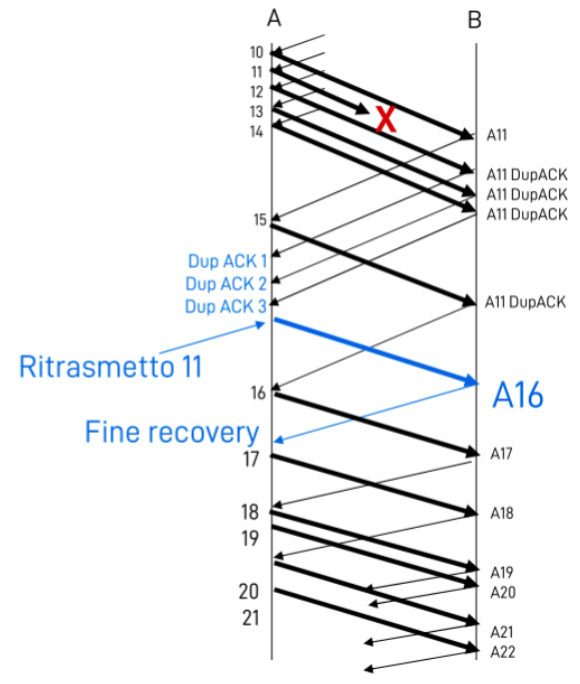
\includegraphics[width=\textwidth]{fast-recovery-esempio.png}
    \end{minipage}
    
    \noindent
    Successivamente vengono ricevuti gli $ACK11$ duplicati e, all'arrivo
    del terzo duplicato, cioè dell'ACK associato al segmento 14,
    il mittente ritrasmette il segmento 11 ed entra in Fast Recovery:
    \begin{itemize}
        \item $\text{RECOVER}=14$;
        \item $\text{SSTHRESH}=\frac{CWND}{2}=2$;
        \item $\text{CWND}=\text{SSTHRESH}+3=5$;
        \item $W_T=[11,\,\dots,\,15]$;
    \end{itemize}
    Quando il destinatario riceve il segmento 15 risponde con un quarto
    $ACK11$ che fa aumentare di una MSS la CWND del mittente, il quale può
    quindi procedere a trasmettere il segmento 16.

    Contemporaneamente, il destinatario ha ricevuto il segmento 11 e
    quindi può confermare anche la ricezione di tutti i segmenti successivi
    già ricevuti: risponde con $ACK16$.

    Il mittente riceve $ACK16$ e poiché include RECOVER, passa in Congestion
    Avoidance e imposta CWND a SSTHRESH, cioè a 2. $W_{LOW}$ viene spostato a
    16, quindi $W_T=[16,\,17]$.
\end{eg}

\begin{figure}[ht]
    \centering
    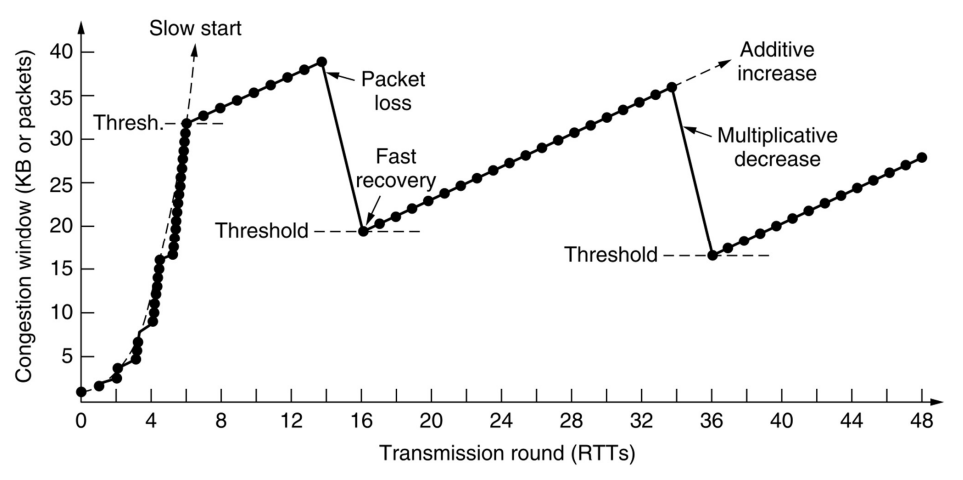
\includegraphics[width=0.8\textwidth]{fast-recovery-grafico.png}
    \caption{\emph{TCP} con \emph{fast retransmit} e \emph{fast recovery}}
\end{figure}
\begin{note}
    Nella figura sottostante gli istanti nei quali il \emph{TCP} si trova in
    \emph{fast recovery} non sono mostrati.
\end{note}
\newpage
\paragraph{Macchina a stati dell'algoritmo AIMD}
L'algoritmo \emph{AIMD} può essere efficacemente descritto come una macchina a
stati:
\begin{figure}[h!]
    \centering
    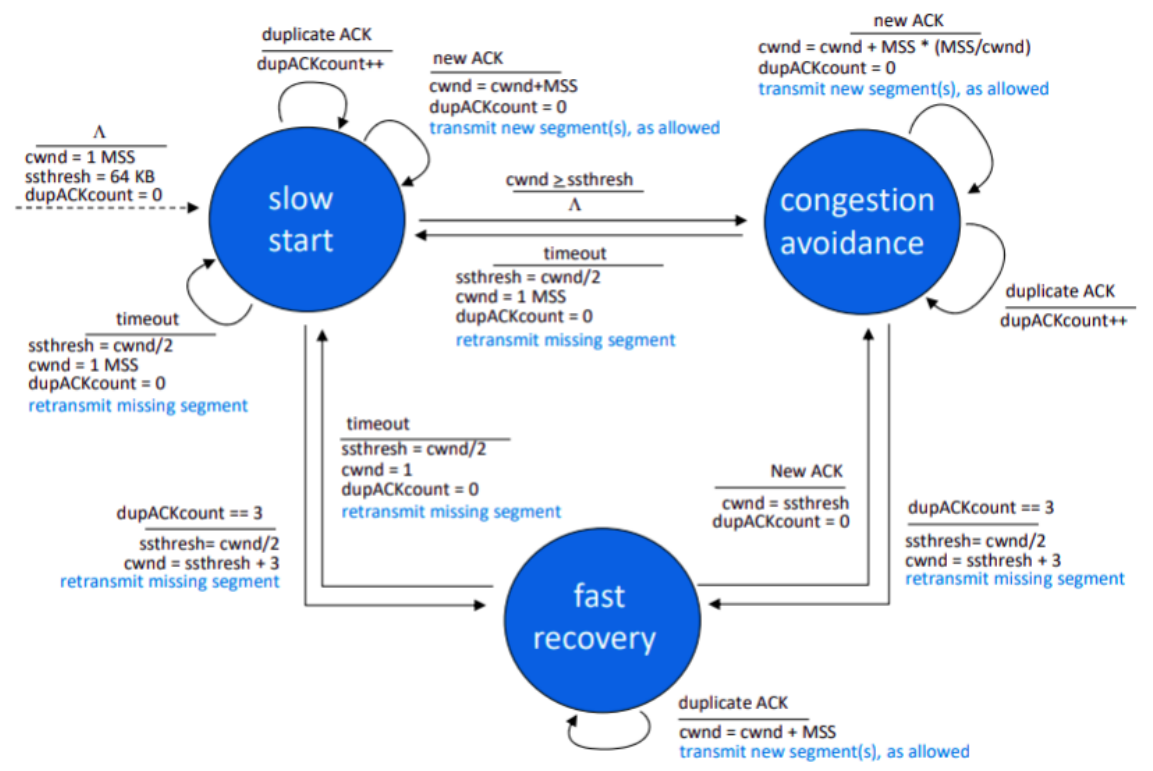
\includegraphics[width=0.95\textwidth]{aimd-macchina-stati.png}
    \caption{Macchina a stati dell'algoritmo \emph{AIMD}}
\end{figure}

\paragraph{Calcolo del throughput}
La seguente formula:
\[Thr(RTT,p)<\frac{MSS}{RTT}\cdot\frac{1}{\sqrt{p}}\]
permette di calcolare il limite superiore al \emph{throughput} del \emph{TCP}.
Il parametro $p$ indica la probabilità di perdere un \emph{segmento}.

\paragraph{Problemi di fairness}
Il protocollo \emph{TPC}, in realtà, non risolve del tutto i problemi di
\emph{fairness} e i motivi sono principalmente due:
\begin{enumerate}
    \item Le applicazioni multimediali, o in generale le applicazioni che
    tollerano delle perdite, utilizzando il protocollo \emph{UDP} per la
    trasmissione dei \emph{segmenti}. Poiché il protocollo \emph{UDP} non
    ha un meccanismo di \emph{controllo della congestione}, è probabile che
    le comunicazioni \emph{TCP} diminuiscano il \emph{throughput};
    \item Le applicazioni possono aprire più connessioni \emph{TCP} in
    parallelo tra due \emph{host} e quindi, se due applicazioni condividono
    lo stesso collegamento, ma una ha aperto una sola connessione, mentre
    l'altra più di una, il \emph{throughput} della prima risulterà inferiore
    al \emph{throughput} complessivo della seconda.
\end{enumerate}

\section{Versioni moderne del TCP}
La versione di \emph{TCP} che abbiamo visto e che usava \emph{AIMD} come
protocollo per il \emph{controllo della congestione} era \emph{loss-based},
ovvero decideva la frequenza di invio dei \emph{segmenti} basandosi soltanto
su quelli persi. Tuttavia, esistono algoritmi più moderni che cercano di
basarsi sul livello di \emph{congestione} effettivo della rete.

\subsection{Protocollo CUBIC}
Il protocollo \emph{CUBIC} gestisce la \emph{congestione} facendo variare la
dimensione della \emph{finestra di congestione} basandosi su una funzione
cubica del tempo. Ciò permette di ottenere una migliore scalabilità e
stabilità su reti veloci e a lunga distanza.

In particolare, \emph{CUBIC} utilizza entrambi i profili, concavo e convesso,
di una funzione cubica per aumentare la dimensione della \emph{finestra di
congestione} e, in reti con \emph{RTT} brevi, è progettato per comportarsi
come il \emph{TCP} standard. Questa adattabilità è realizzata impostando
opportunamente il \emph{coefficiente di diminuzione} della \emph{finestra di
congestione} che è $0.5$ nel \emph{TCP} standard (la \emph{finestra} viene
dimezzata) e $0.7$ nel \emph{CUBIC}.

\begin{figure}[hb]
    \centering
    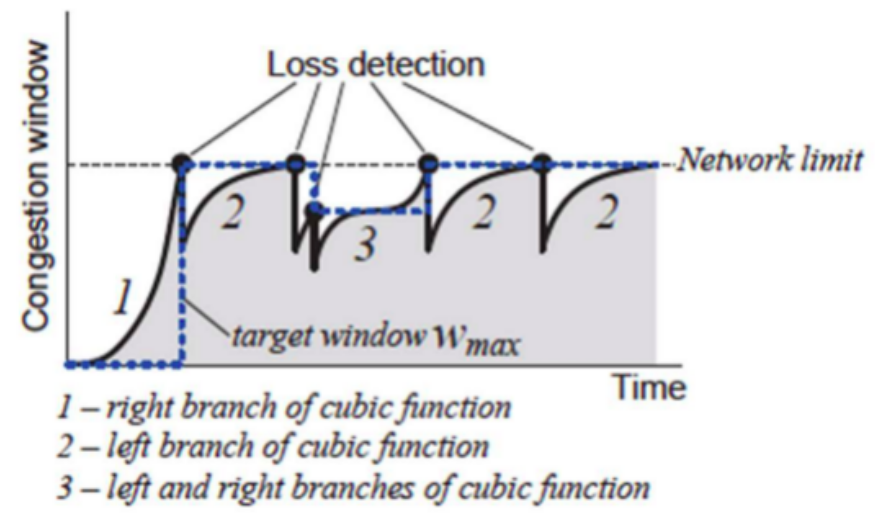
\includegraphics[width=0.8\textwidth]{cubic.png}
    \caption{\emph{TCP CUBIC}}
\end{figure}

\subsection{Protocollo BBR}
\emph{\gls{prot:BBR}} è un protocollo server-side sviluppato da Google nel 2016
e invece di basarsi sulle perdite, sfrutta due parametri, quali la \emph{banda}
del collegamento che funge da collo di bottiglia e l'\emph{RTT}, per modulare la
velocità di trasmissione dei \emph{segmenti}. L'idea alla base del \emph{BBR}
è proprio riuscire a trasmettere i \emph{segmenti} ad una velocità tale da
evitare che si creino accodamenti.

\begin{note}
    Il fatto che sia un protocollo \emph{server-side} fa si che non sia
    necessario implementare \emph{BBR} anche sui client.
\end{note}\noindent
Il \emph{BBR} inizia a trasmettere aumentando esponenzialmente il numero
di \emph{segmenti} trasmessi. Quando vede che i \emph{segmenti} iniziano ad
accodarsi, smette di trasmettere e aspetta fino allo smaltimento della coda.
A questo punto, continua a trasmettere ad una frequenza alla quale non si
creano accodamenti e tenta, ogni tanto, di incrementarla. Se
l'incremento viene sostenuto dalla rete, cioè se continuano a non
formarsi code, mantiene la frequenza aumentata, altrimenti ritorna a quella
precedente. Questo ciclo si ripete periodicamente.

Un'altra cosa che il \emph{BBR} fa periodicamente, è smettere di trasmettere
e aspettare che la coda si svuoti del tutto. A quel punto trasmette
un \emph{segmento} e ne misura l'\emph{RTT}. L'\emph{RTT} misurato in quella
situazione ideale viene impostato come \emph{RTT} minimo.

\begin{figure}[h!]
    \centering
    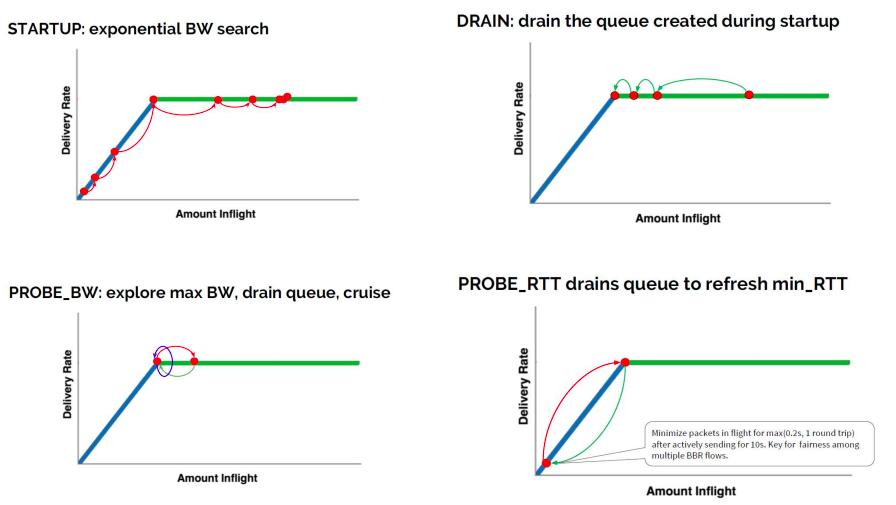
\includegraphics[width=\textwidth]{bbr.png}
    \caption{\emph{TCP BBR}}
\end{figure}\noindent
Secondo Google, il \emph{BBR} permette di ottenere un \emph{throughput} di
circa $9100Mbit/s$ contro i $3.3Mbit/s$ del \emph{CUBIC}. Inoltre, per
le sue caratteristiche, il \emph{BBR} è ottimo se combinato con l'\emph{HTTP/2.0}
e se utilizzato per raggiungere le cosiddette \quotes{reti di ultimo miglio}.

\begin{figure}[t]
    \centering
    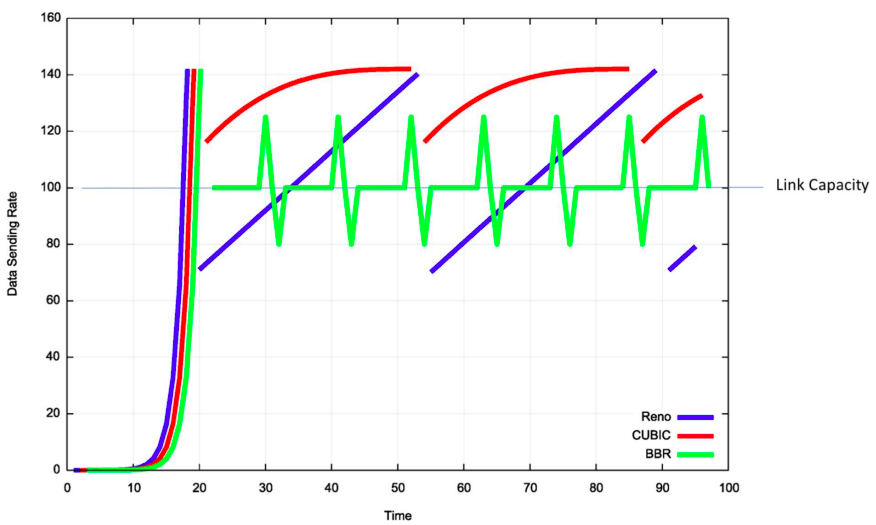
\includegraphics[width=0.7\textwidth]{reno-cubic-bbr.png}
    \caption{\emph{Reno} VS \emph{CUBIC} VS \emph{BBR}} 
\end{figure}
\begin{note}
    \emph{Reno} è il nome del \emph{TCP} standard.
\end{note}
\newpage
\subsection{Protocollo QUIC}
Il protocollo \emph{\gls{prot:QUIC}} mira ad essere equivalente ad una
connessione \emph{TCP}, ma riducendo l'overhead di connessione e utilizzando
di base il protocollo \emph{UDP} per il trasporto dei \emph{segmenti}.

Il \emph{QUIC} consente di ridurre l'overhead perché permette, nel processo
di \emph{handshake} iniziale, di incoporare anche i dati necessari
all'instaurazione di una sessione \emph{TLS}. In particolare, quando il
client apre una connessione, il messaggio di risposta include anche i dati
necessari all'uso della crittografia in \emph{TLS}. In questo modo si evita
di dover effettuare due \emph{handshake} in successione: quello per il
\emph{TCP} e quello per il \emph{TLS}.

Abbiamo detto però che il \emph{QUIC} utilizza l'\emph{UDP} invece del \emph{TCP}
e, infatti, la trasmissione si svolge attraverso flussi di dati \emph{QUIC} che
sono gestiti indipendentemente gli uni dagli altri. Ogni perdita viene gestita
dal protocollo \emph{QUIC} stesso e non dall'\emph{UDP}.

Nel caso di cambi di rete, il protocollo \emph{TCP} richiede la restaurazione
di ogni connessione precedentemente utilizzata. Il \emph{QUIC} invece, include un
identificativo di connessione al server che è indipendente dalla fonte o dalla
rete usata. Questo identificativo è memorizzato nel server e può essere usato
dal client per ristabilire la connessione precedentemente inizializzata
semplicemente inviando un \emph{segmento} contenente quell'identificativo.
Ciò permette di azzerare l'overhead necessario a riprendere la comunicazione
dopo un cambio di rete.

\begin{figure}[b]
    \centering
    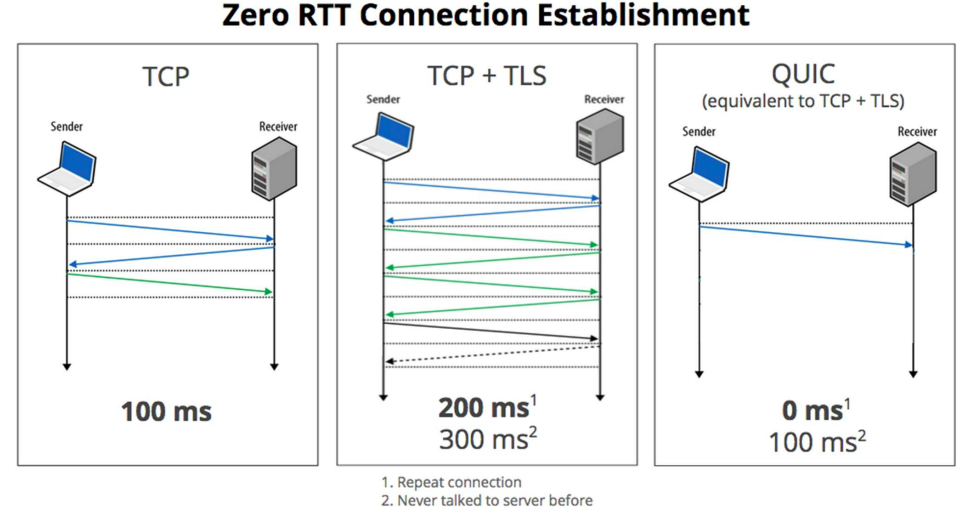
\includegraphics[width=0.7\textwidth]{cuic.png}
    \caption{Tempo necessario ad insitaurare una connessione}
\end{figure}